\section{Performance}
\label{sec:perf}

The MMTP performs admirably.

\subsection{Low-level performance}
\label{sec:perf-simple}

\begin{figure}[!htpb]
  \begin{center}
    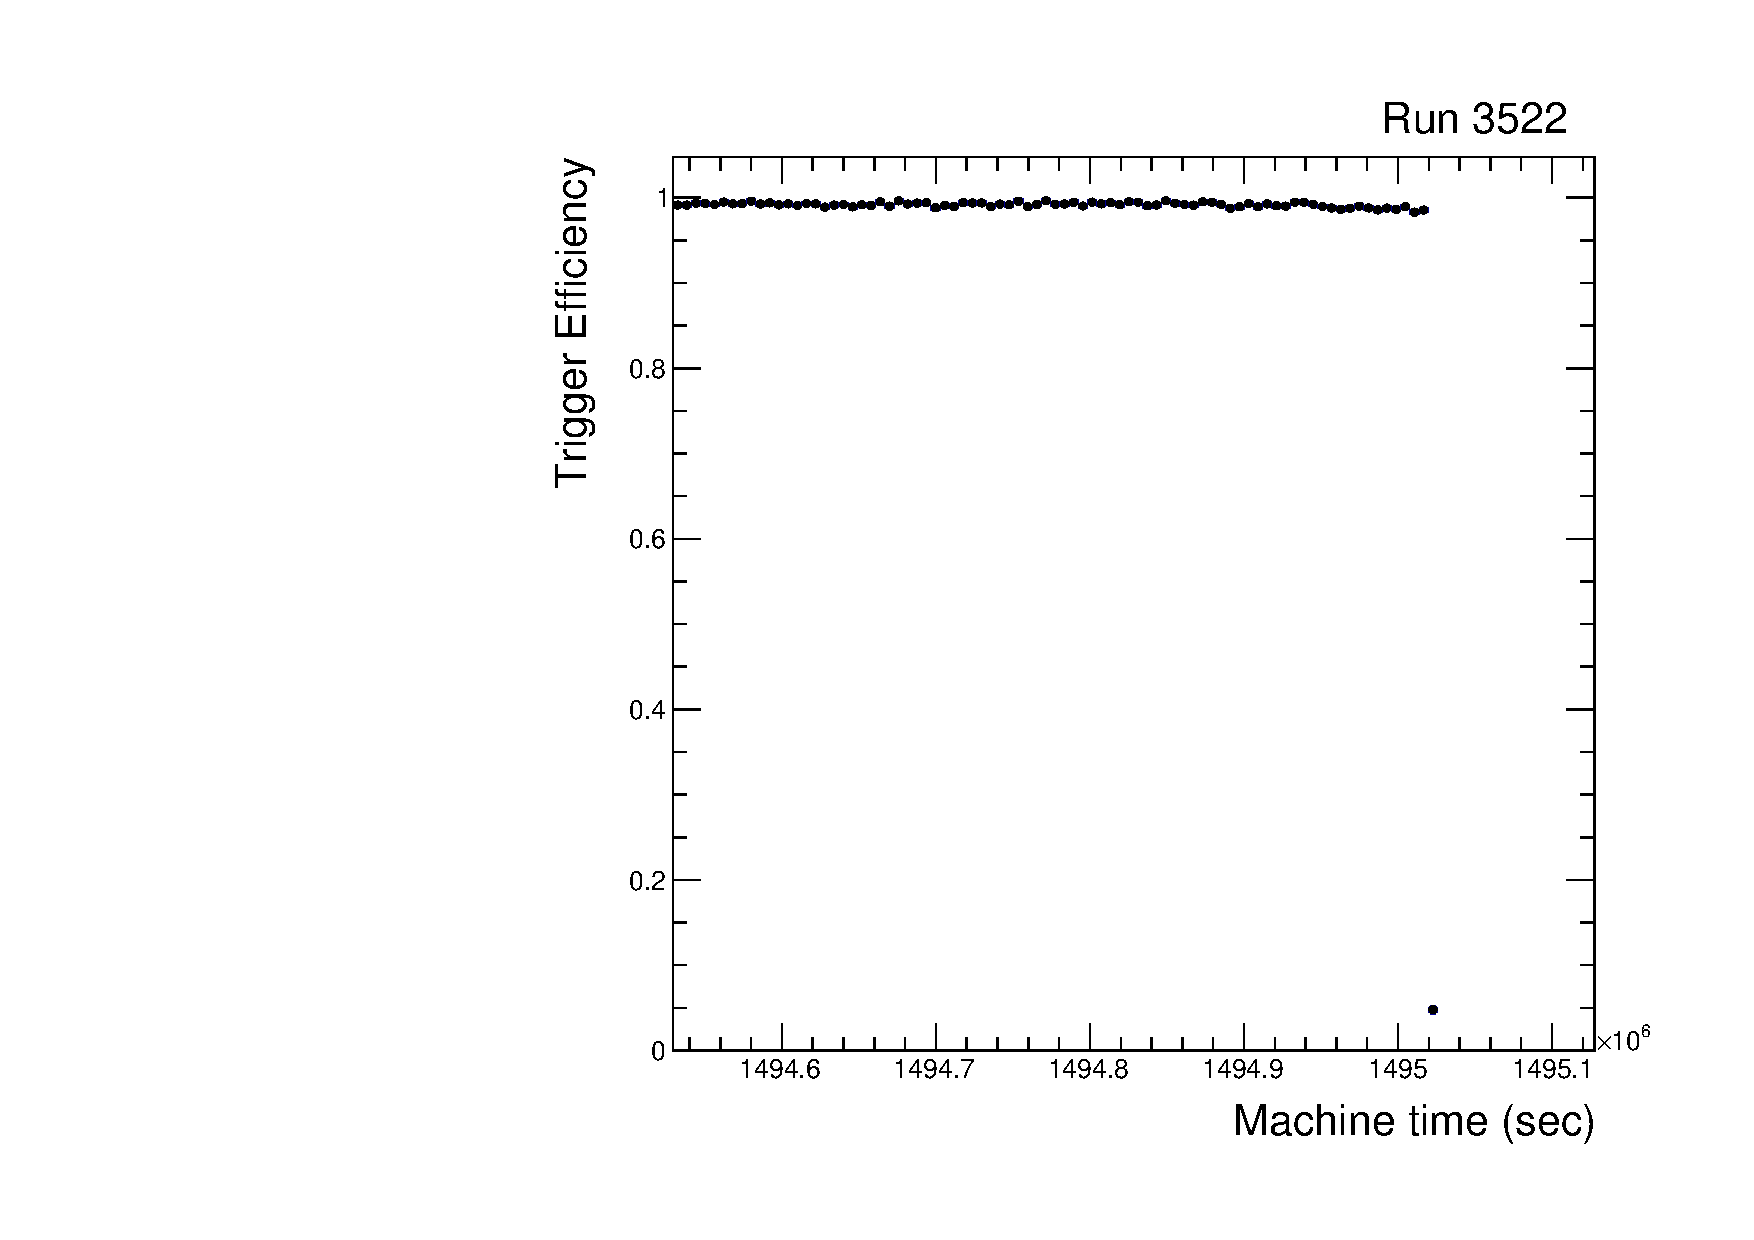
\includegraphics[width=0.4\textwidth]{figures/gbtanalysis3522/tpeff.pdf}
    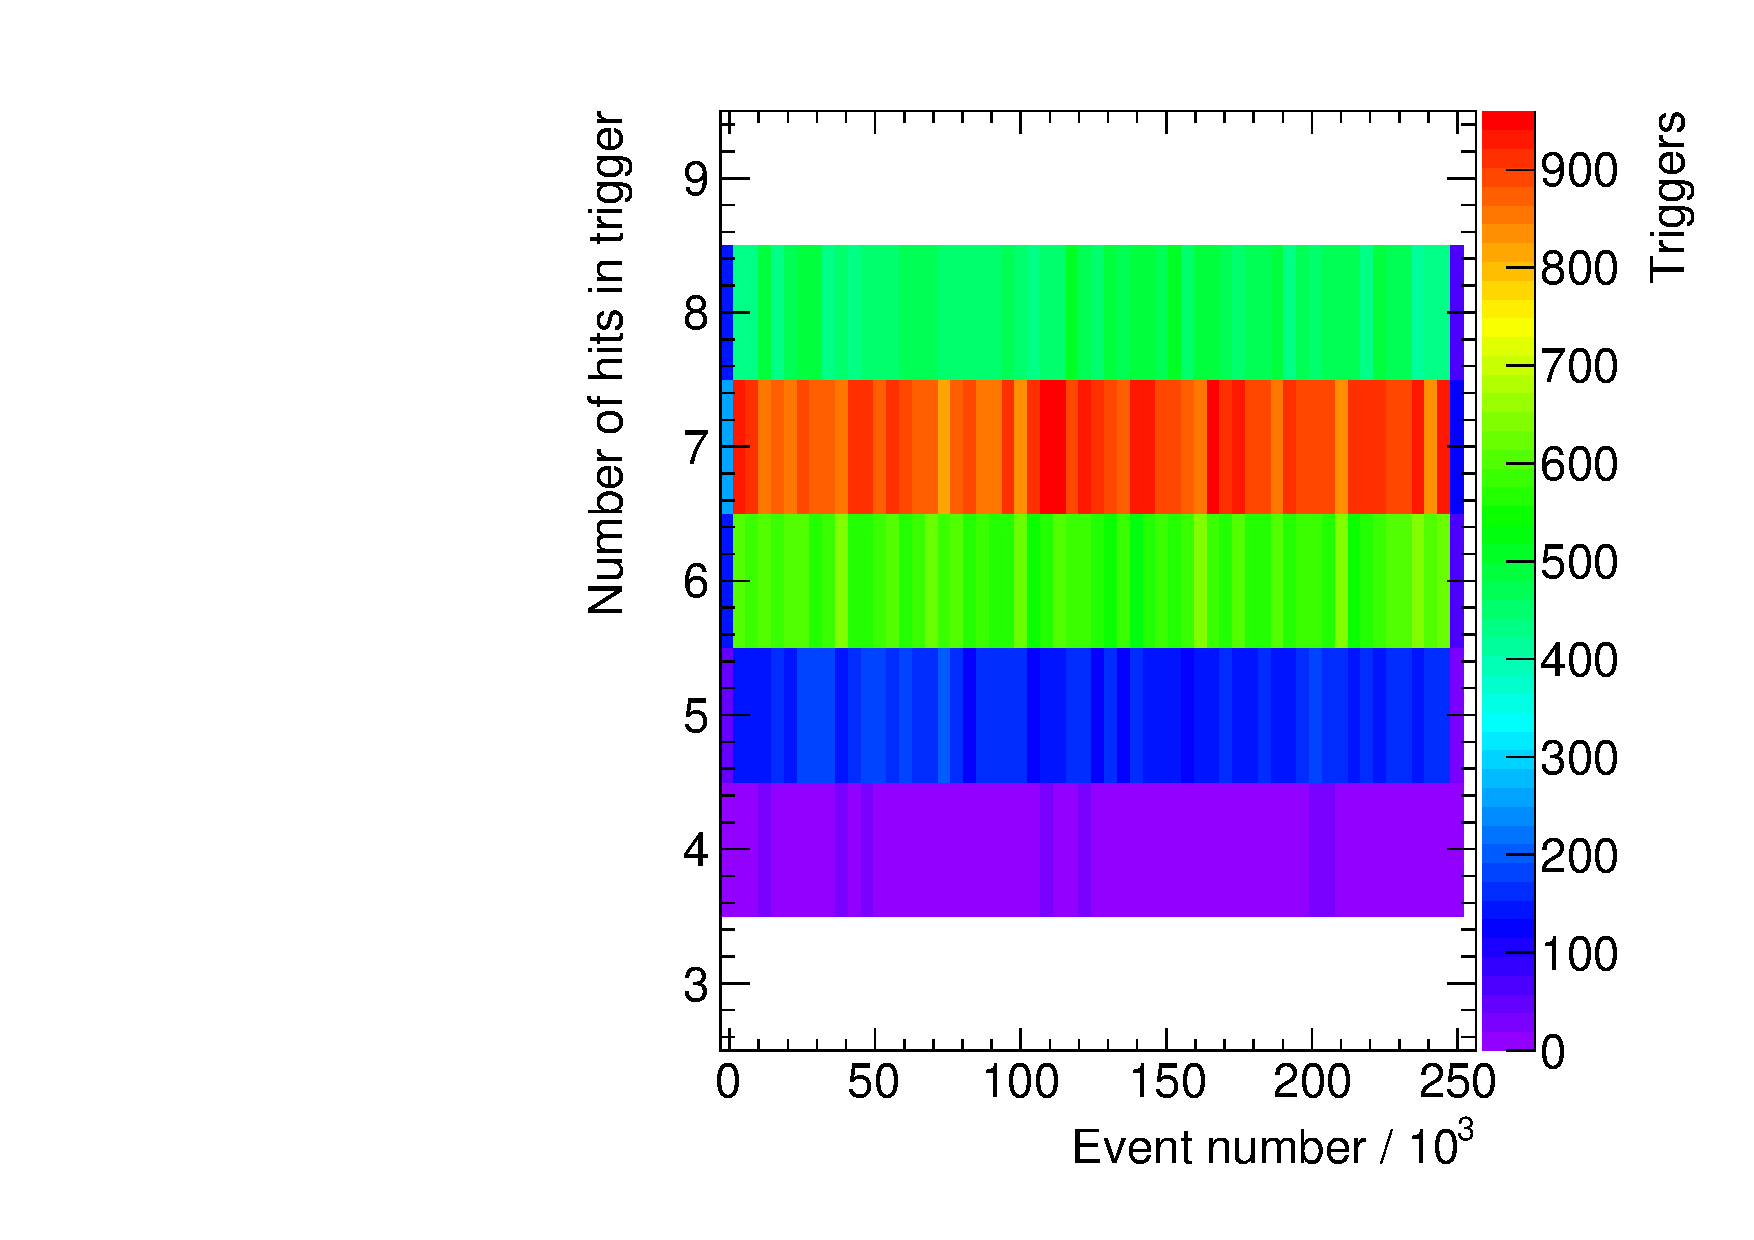
\includegraphics[width=0.4\textwidth]{figures/tuna_analysis/trigger_hits_vs_event.pdf}
  \end{center}
  \vspace{-10pt}
  \caption{The efficiency of a trigger to be matched to a full readout event versus time (left) and the number of hits in the trigger as a function of time (right). Both figures show stable data-taking.}
  \label{fig:lowlevel}
\end{figure}

\begin{figure}[!htpb]
  \begin{center}
    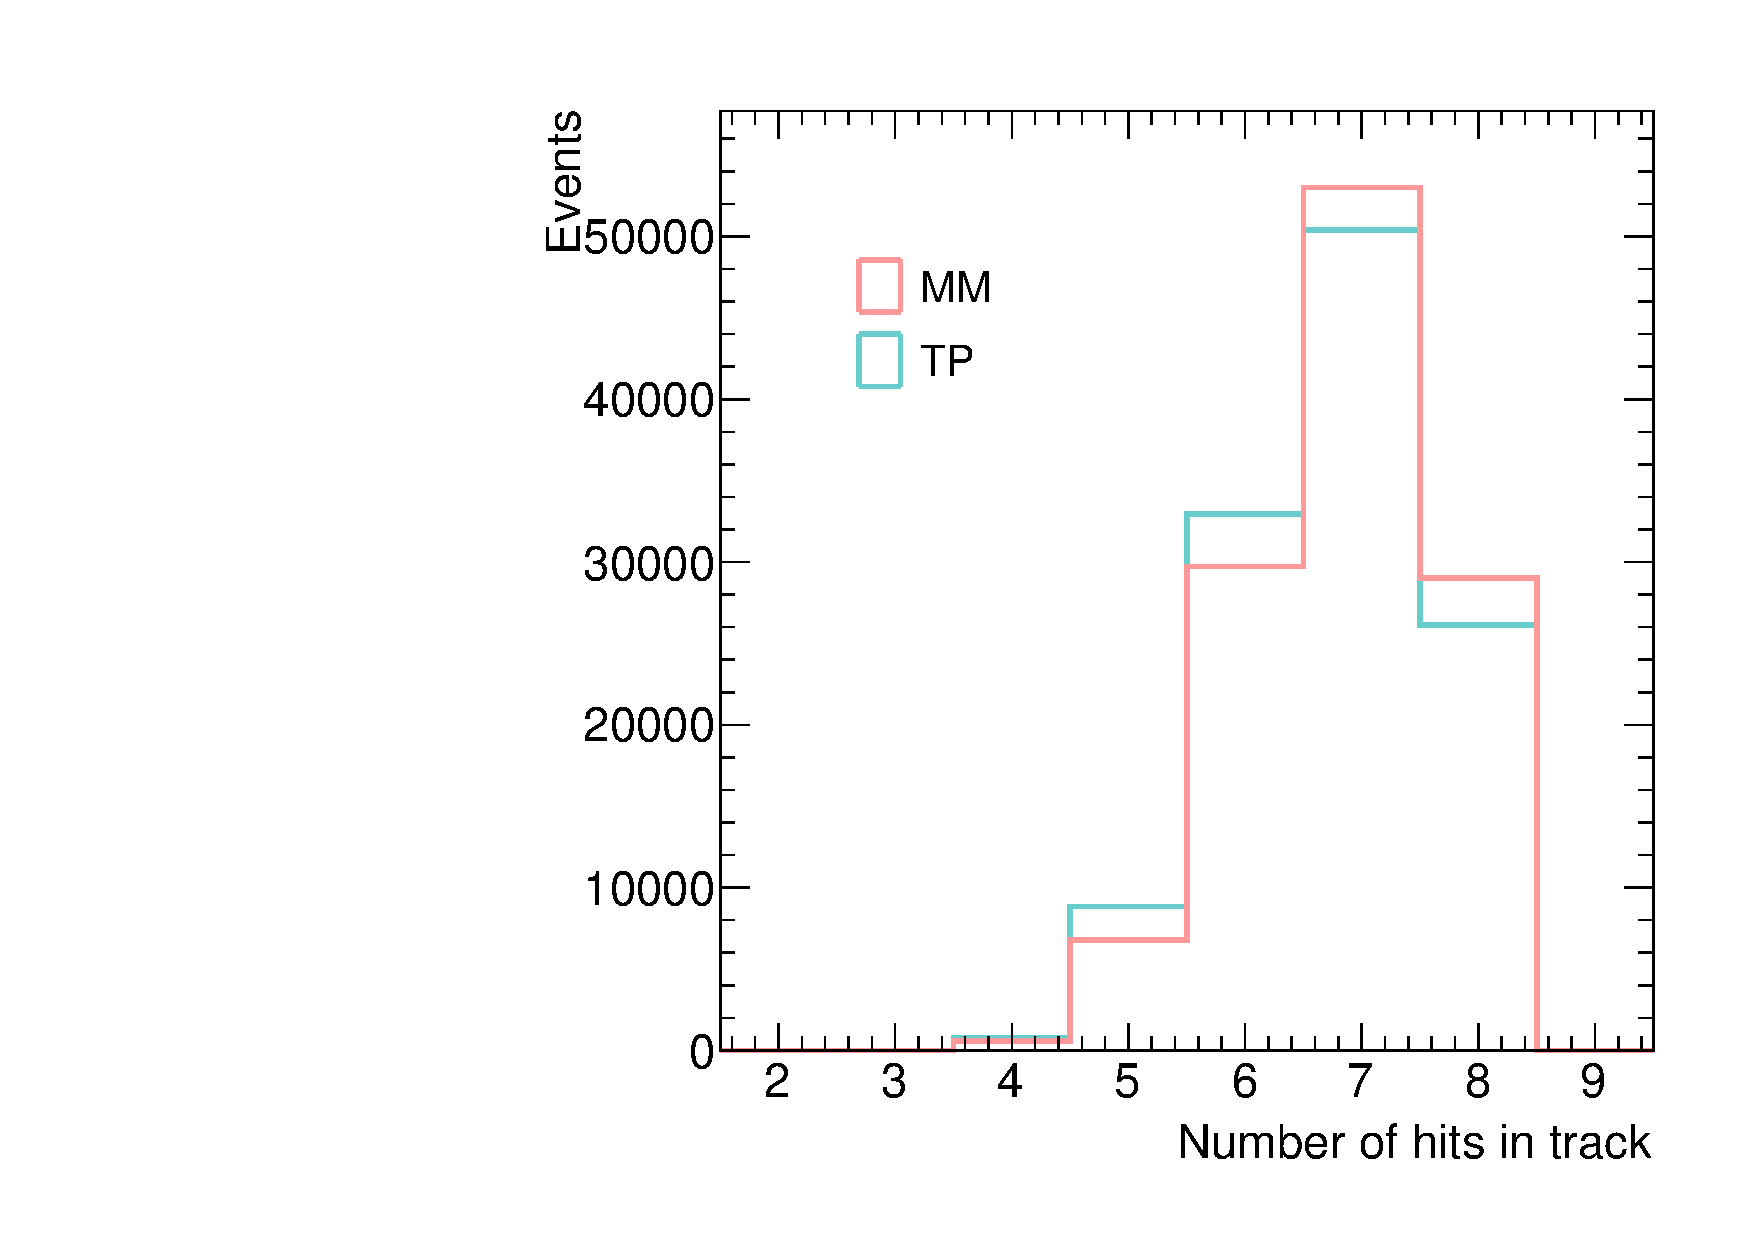
\includegraphics[width=0.4\textwidth]{figures/tuna_analysis/trigger_nart.pdf}
    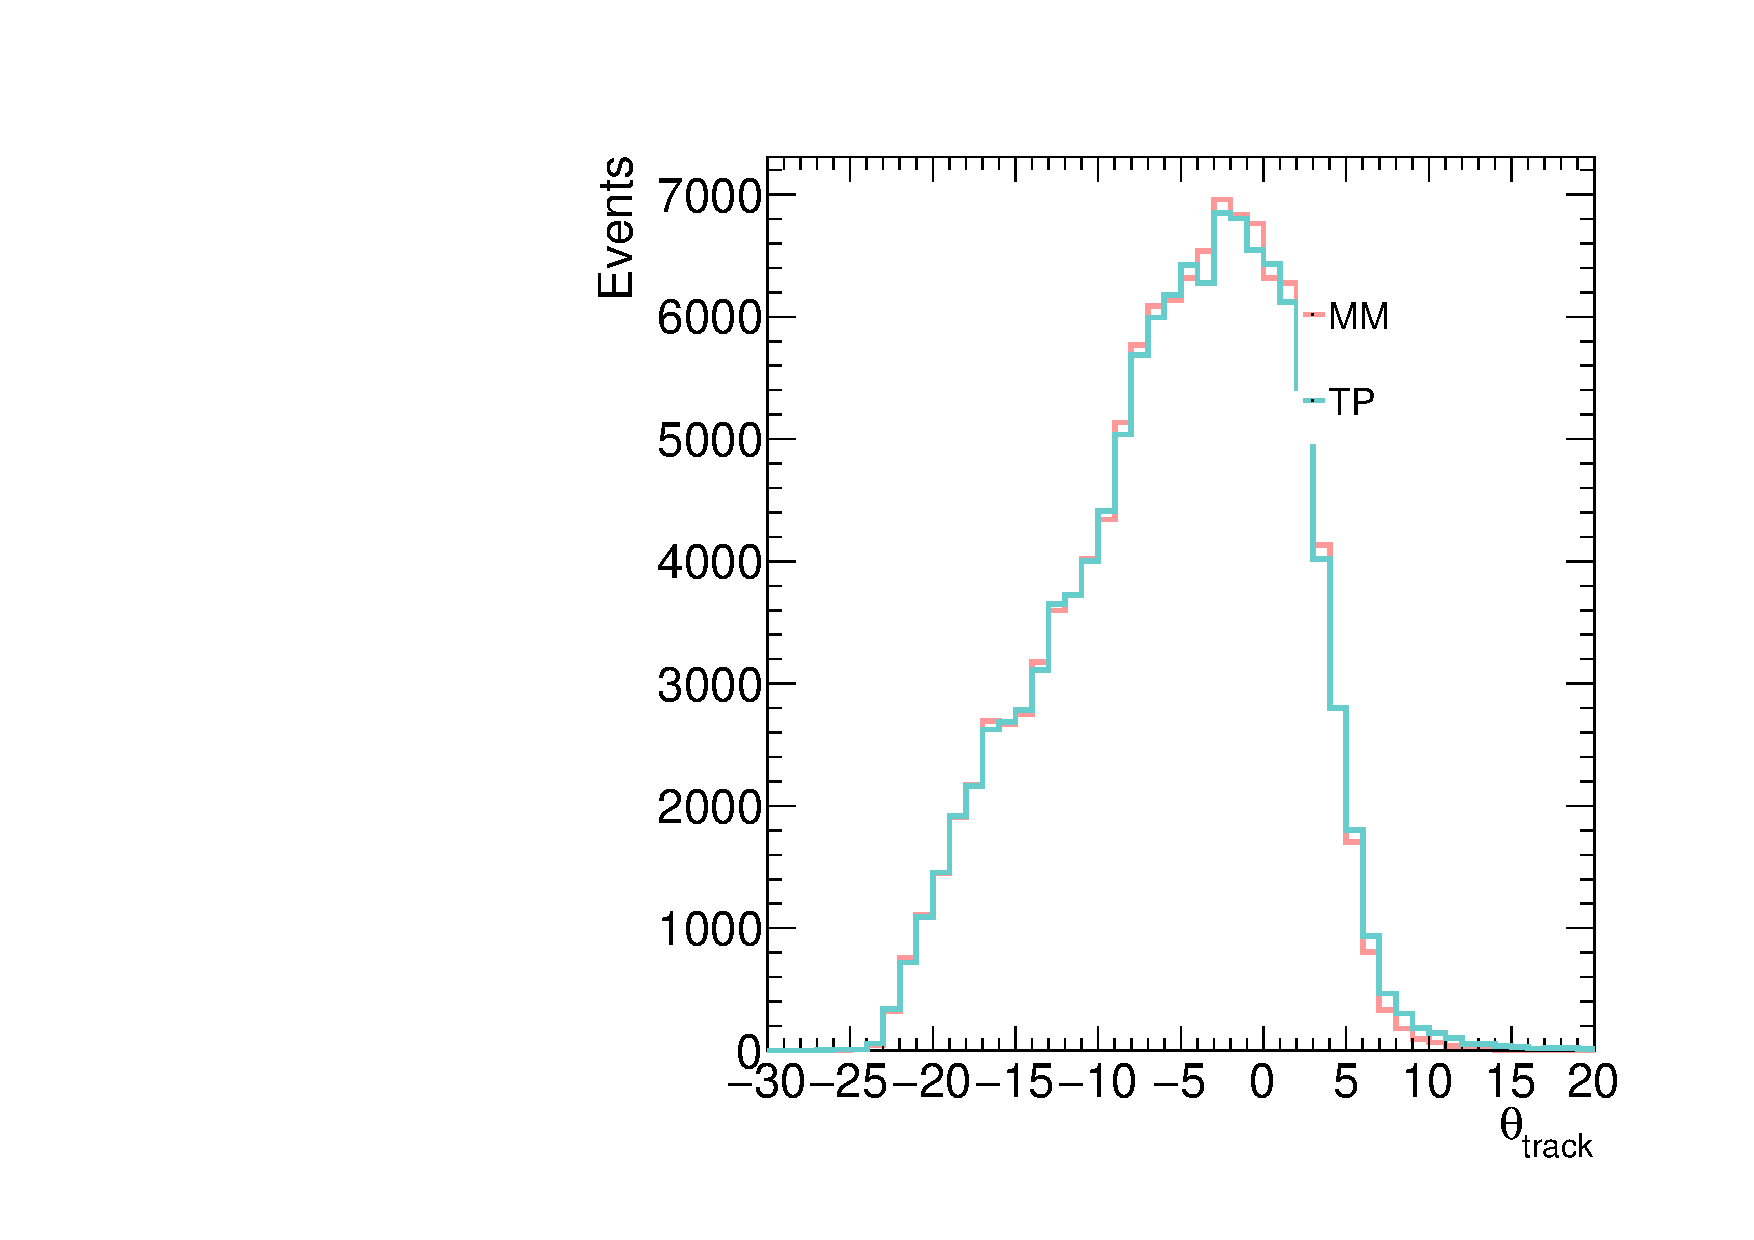
\includegraphics[width=0.4\textwidth]{figures/gbtanalysis3522/ang.pdf}
  \end{center}
  \vspace{-10pt}
  \caption{The number of hits in the MM TP and MM FE tracks (left) and the angle of the tracks (right). The track found by the trigger closely resembles the track found by the full readout, though with slightly fewer hits on average.}
  \label{fig:tp_vs_fe}
\end{figure}

\subsection{Roads}
\label{sec:perf-roads}

\subsection{Spatial and angular resolution}
\label{sec:perf-res}

\begin{figure}[!htpb]
  \begin{center}
    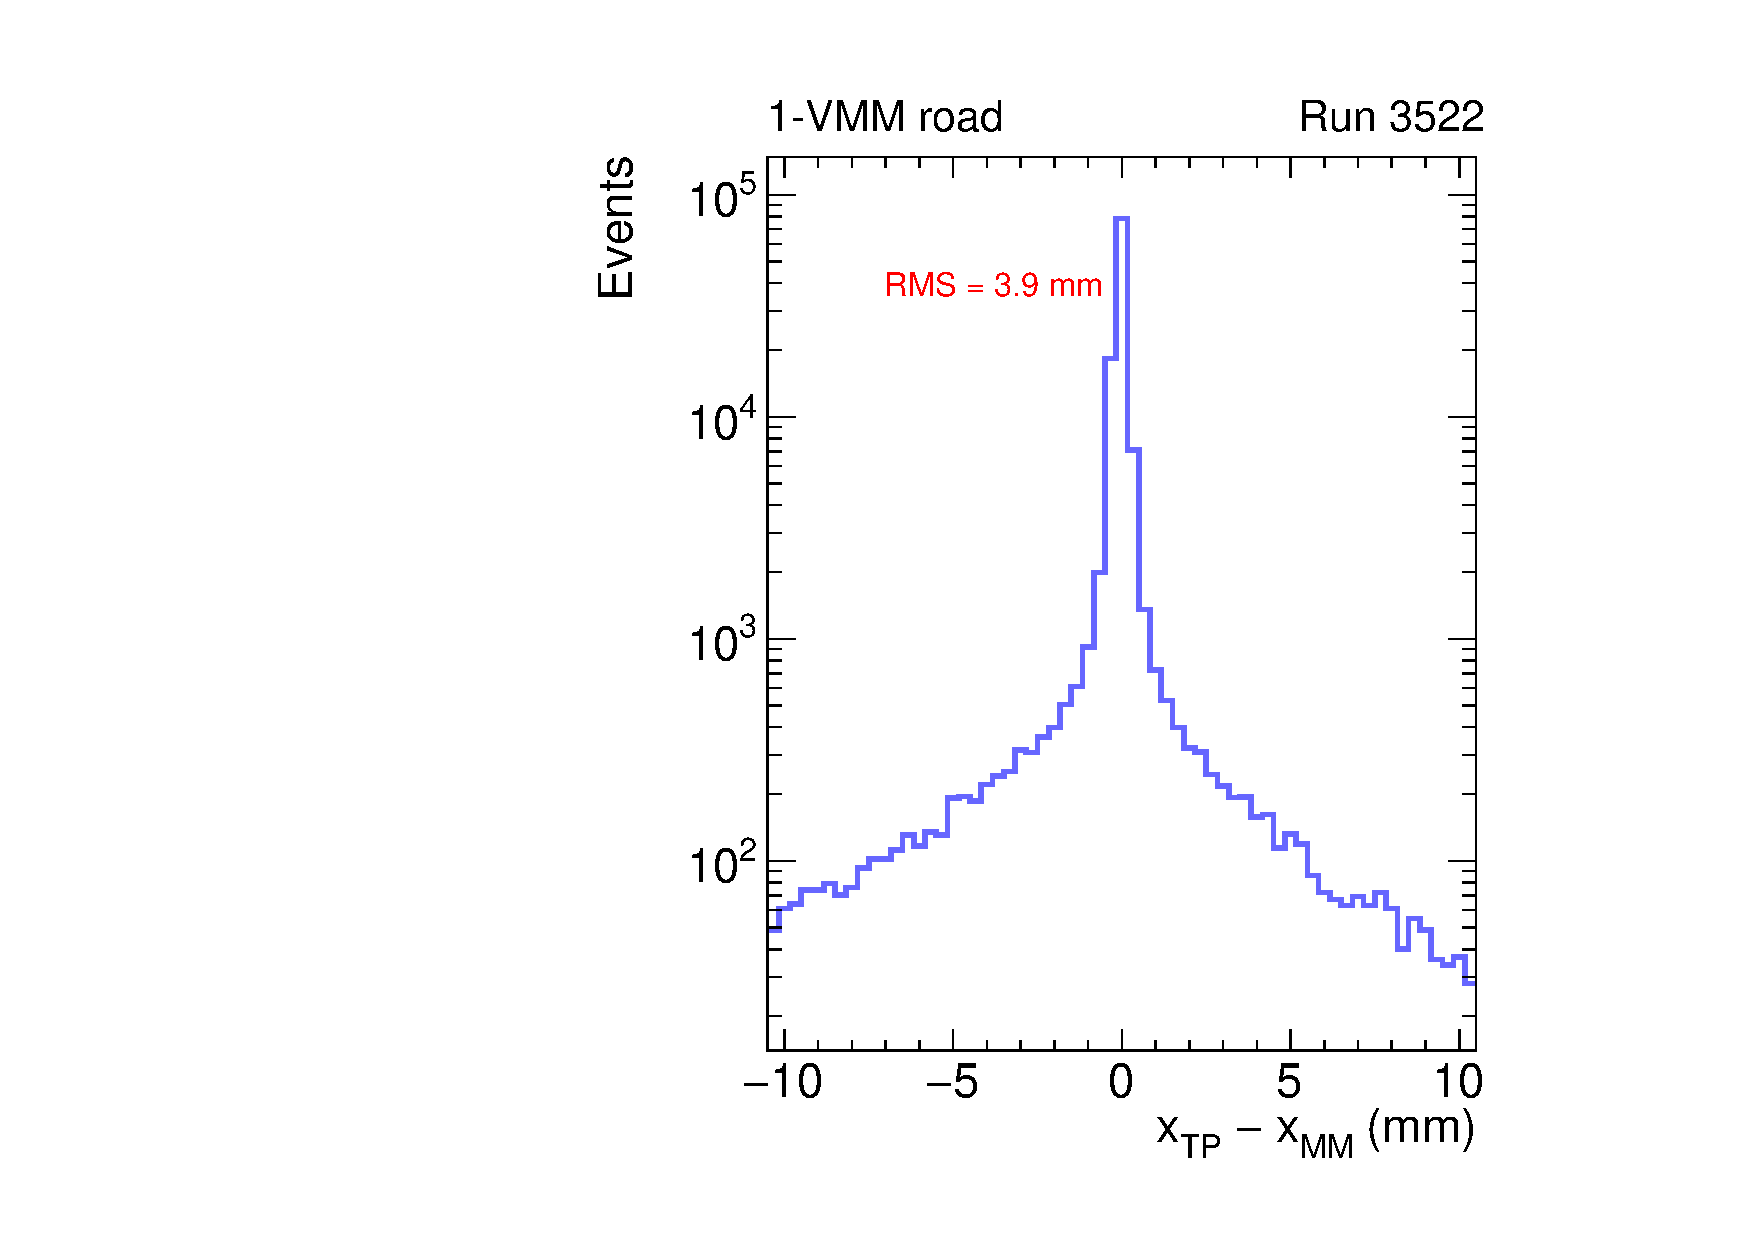
\includegraphics[width=0.4\textwidth]{figures/gbtanalysis3522/TP_xres_full.pdf}
    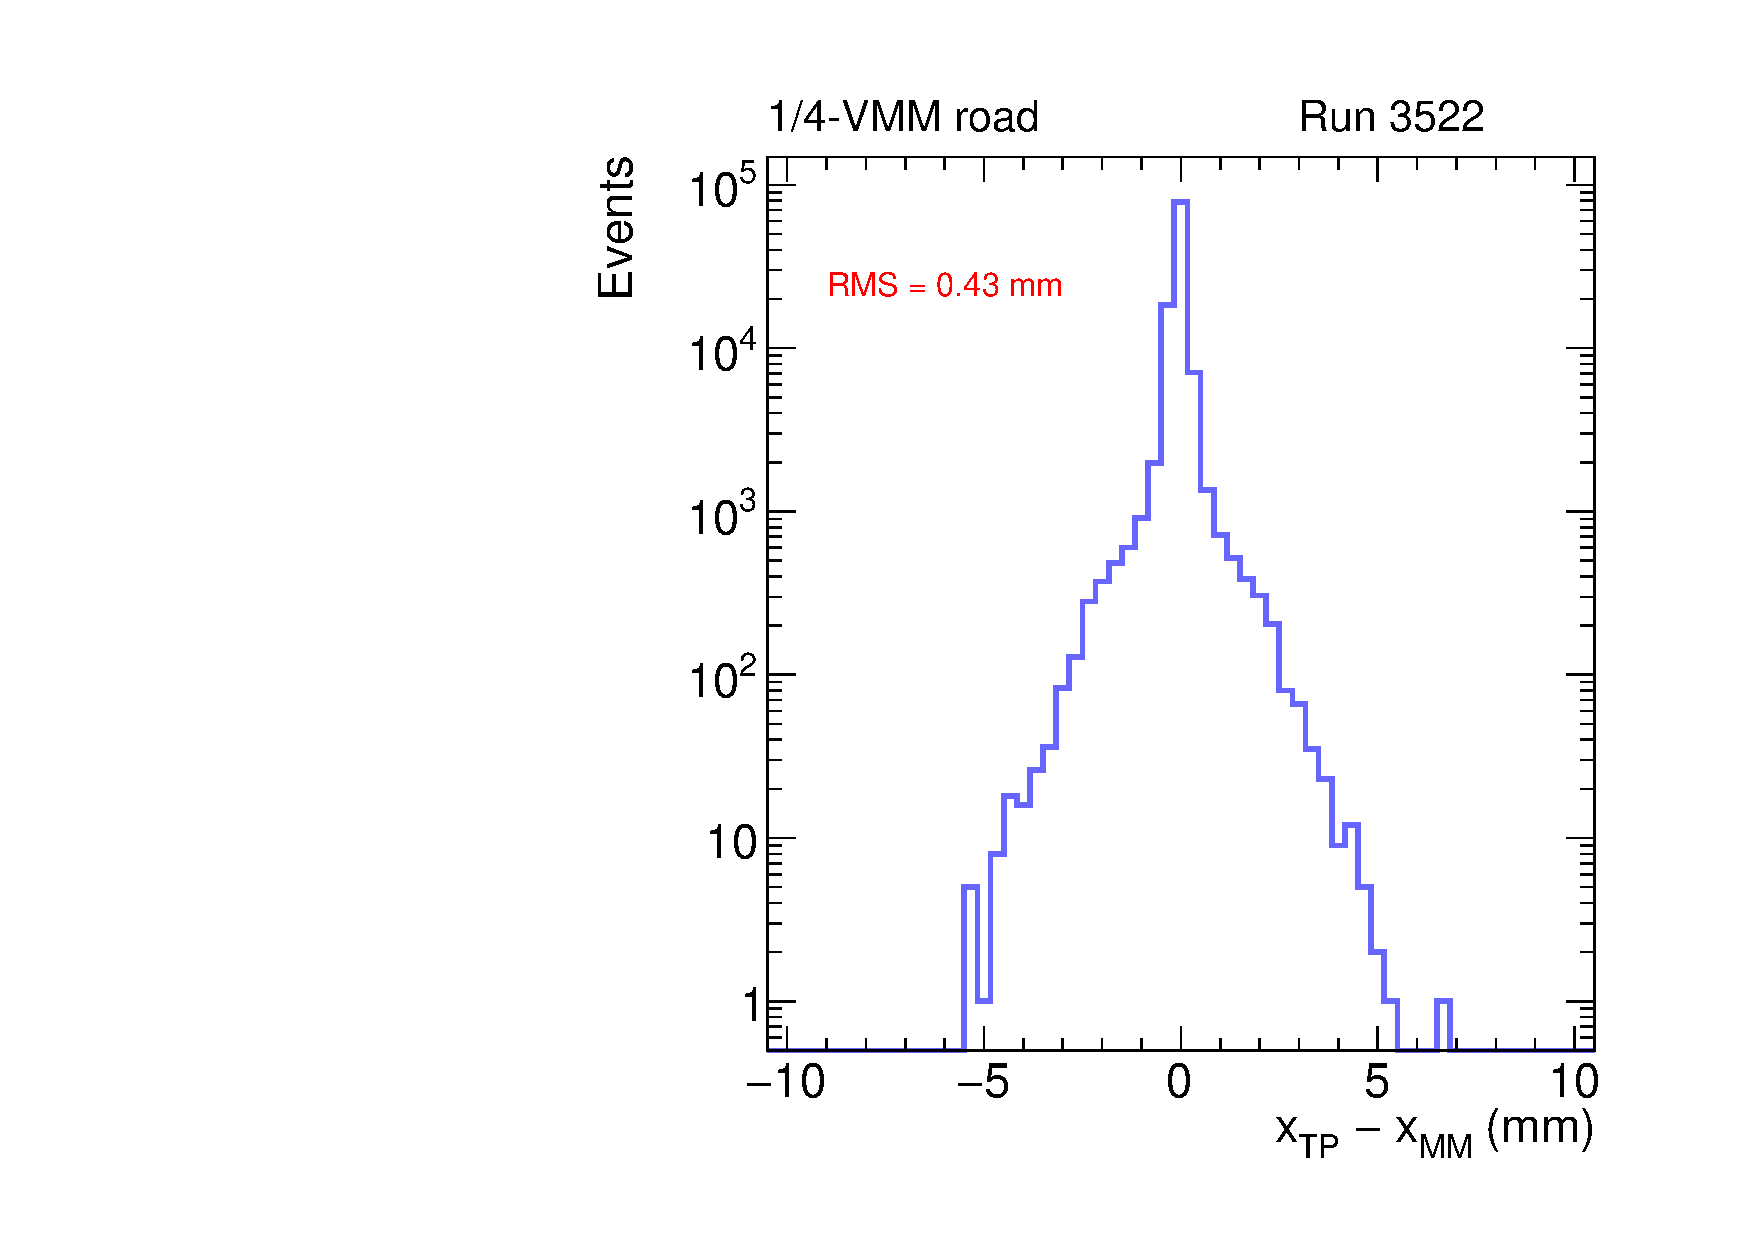
\includegraphics[width=0.4\textwidth]{figures/gbtanalysis3522/TP_xres.pdf}
  \end{center}
  \vspace{-10pt}
  \caption{The $x$ resolution of the MM TP relative to the full readout, using 1-VMM online roads (left) and 1/4-VMM offline roads (right). The tails of the resolution are greatly suppressed with smaller roads.}
  \label{fig:xres}
\end{figure}

\begin{figure}[!htpb]
  \begin{center}
    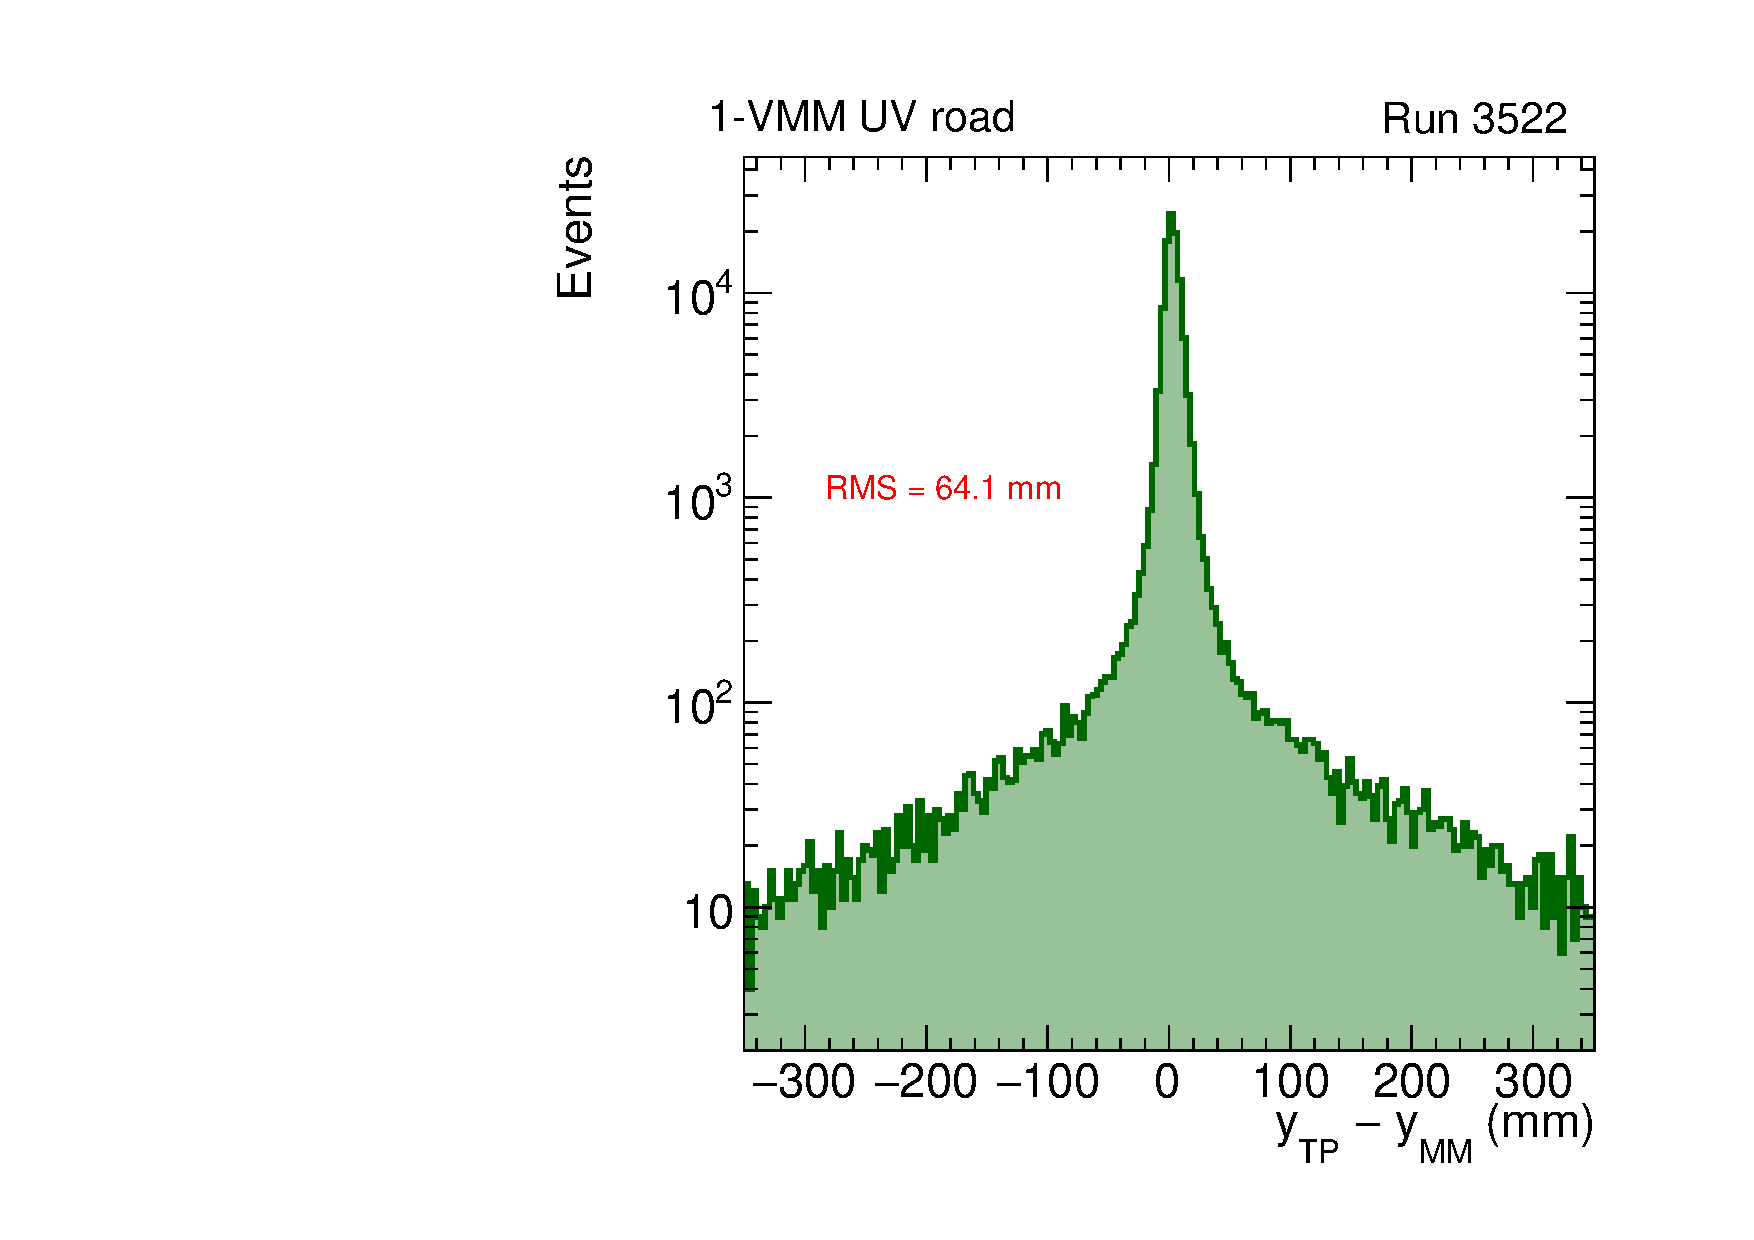
\includegraphics[width=0.4\textwidth]{figures/gbtanalysis3522/TP_yres_1road.pdf}
    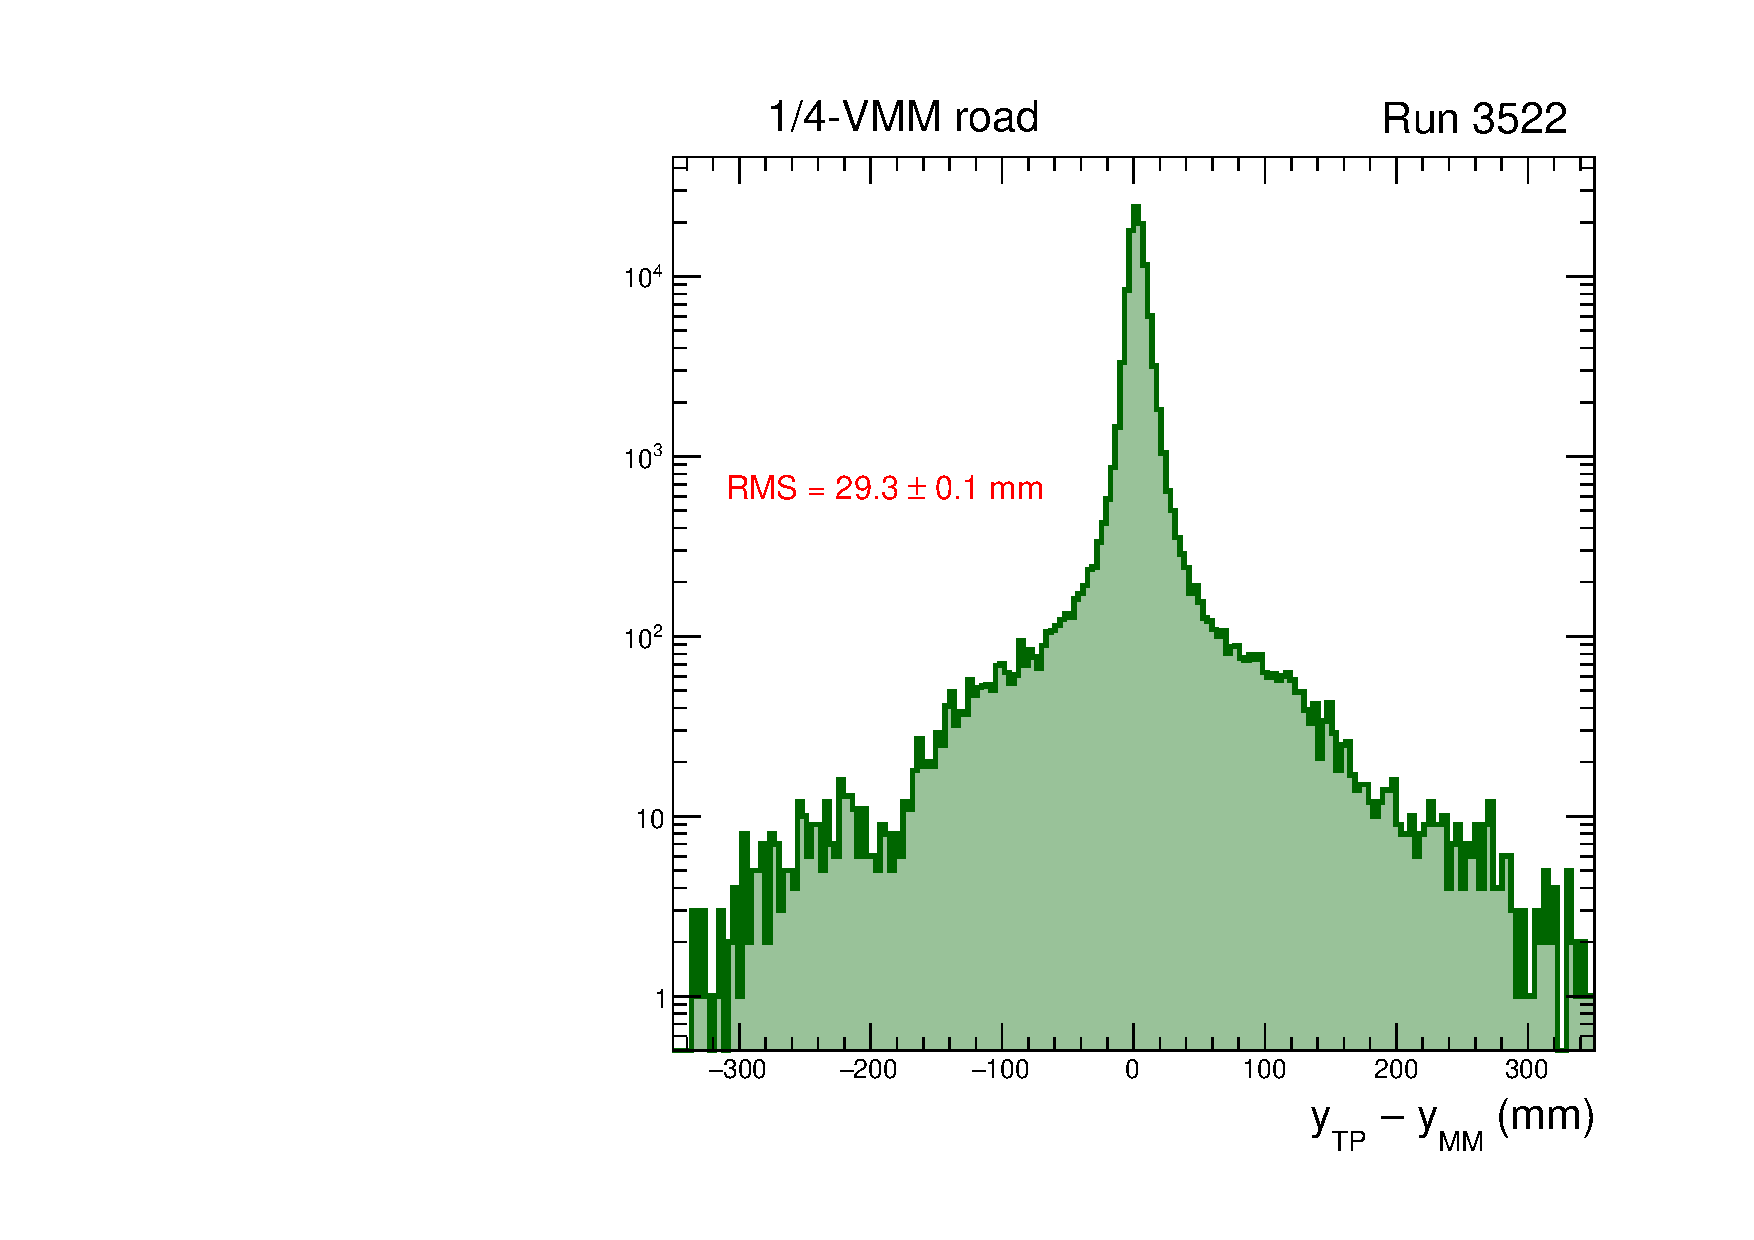
\includegraphics[width=0.4\textwidth]{figures/gbtanalysis3522/TP_yres_smallroad.pdf}
  \end{center}
  \vspace{-10pt}
  \caption{The $y$ resolution of the MM TP relative to the full readout, using 1-VMM online roads (left) and 1/4-VMM offline roads (right). The tails of the resolution are greatly suppressed with smaller roads.}
  \label{fig:yres}
\end{figure}

\begin{figure}[!htpb]
  \begin{center}
    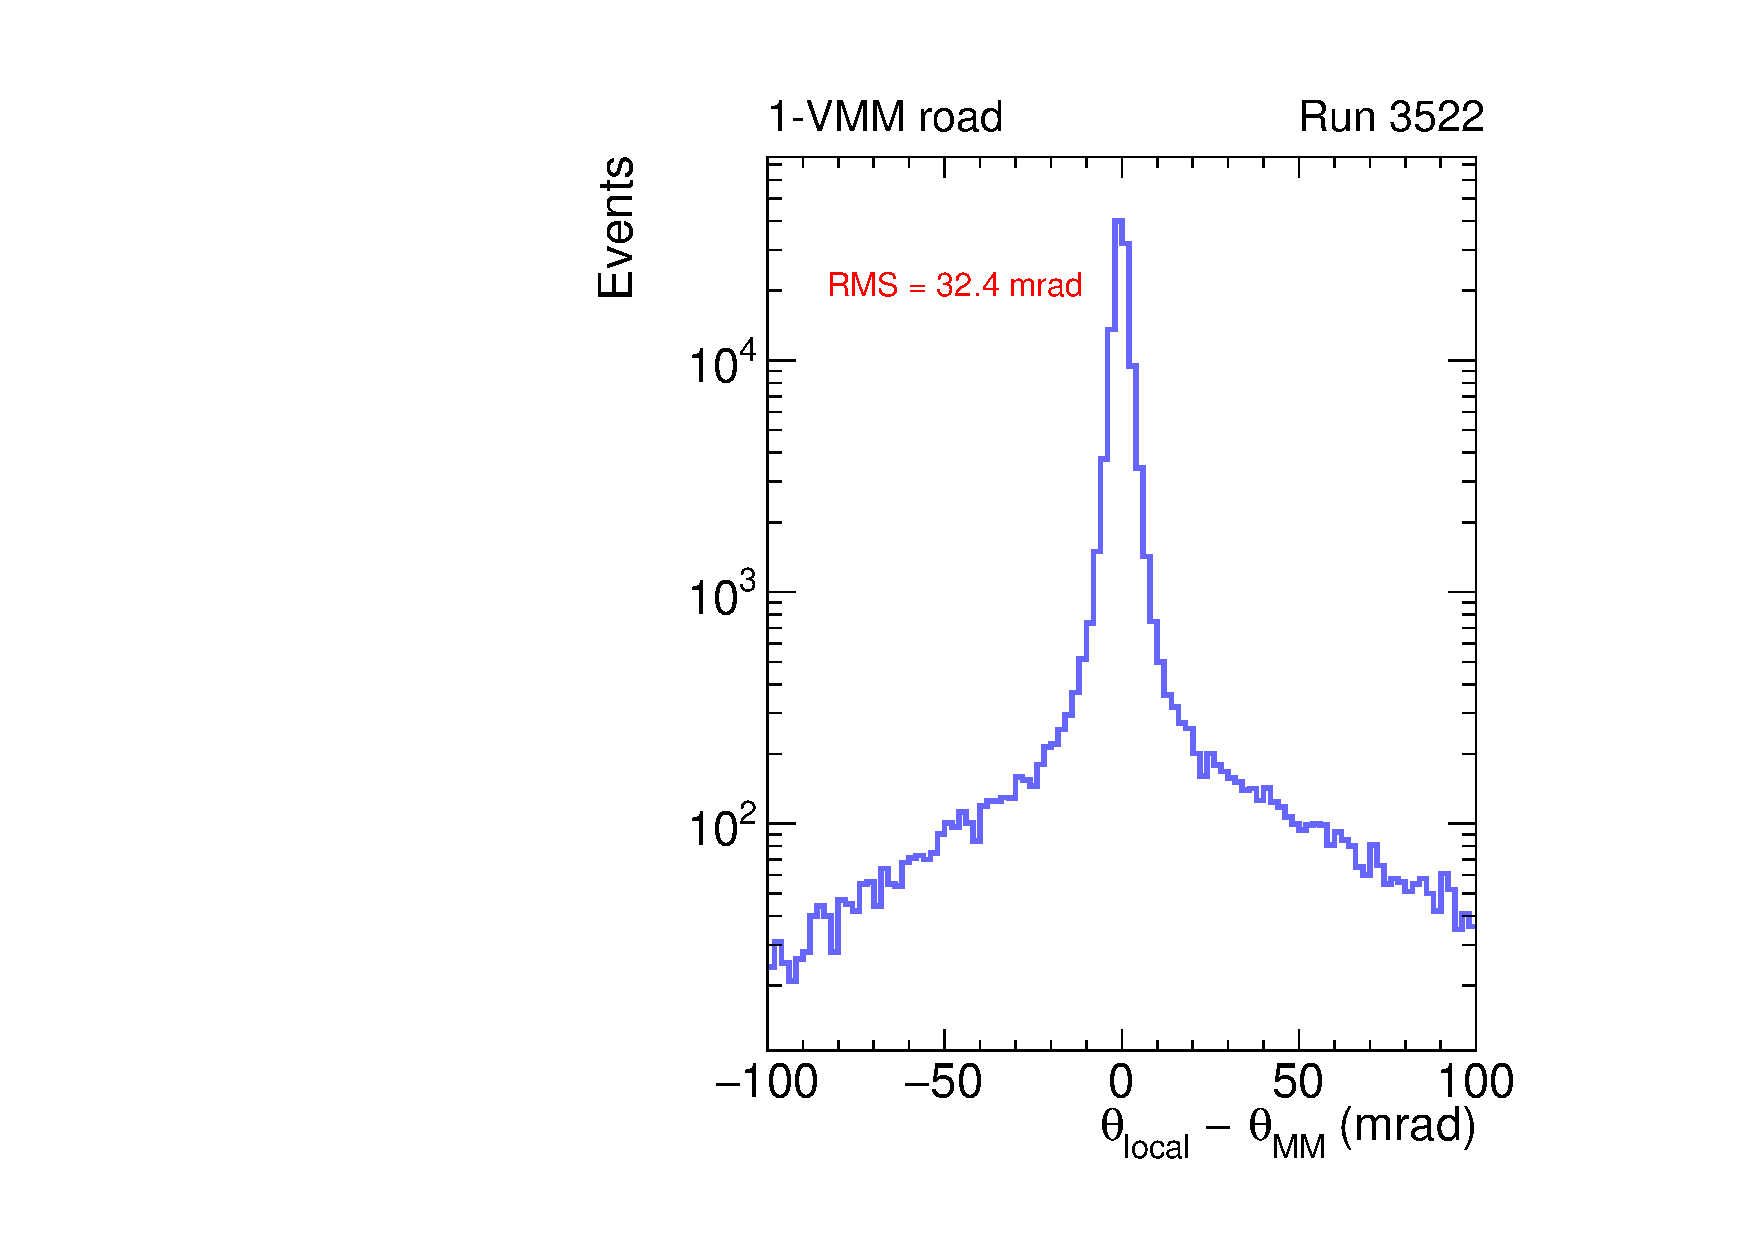
\includegraphics[width=0.4\textwidth]{figures/gbtanalysis3522/TP_angres_full.pdf}
    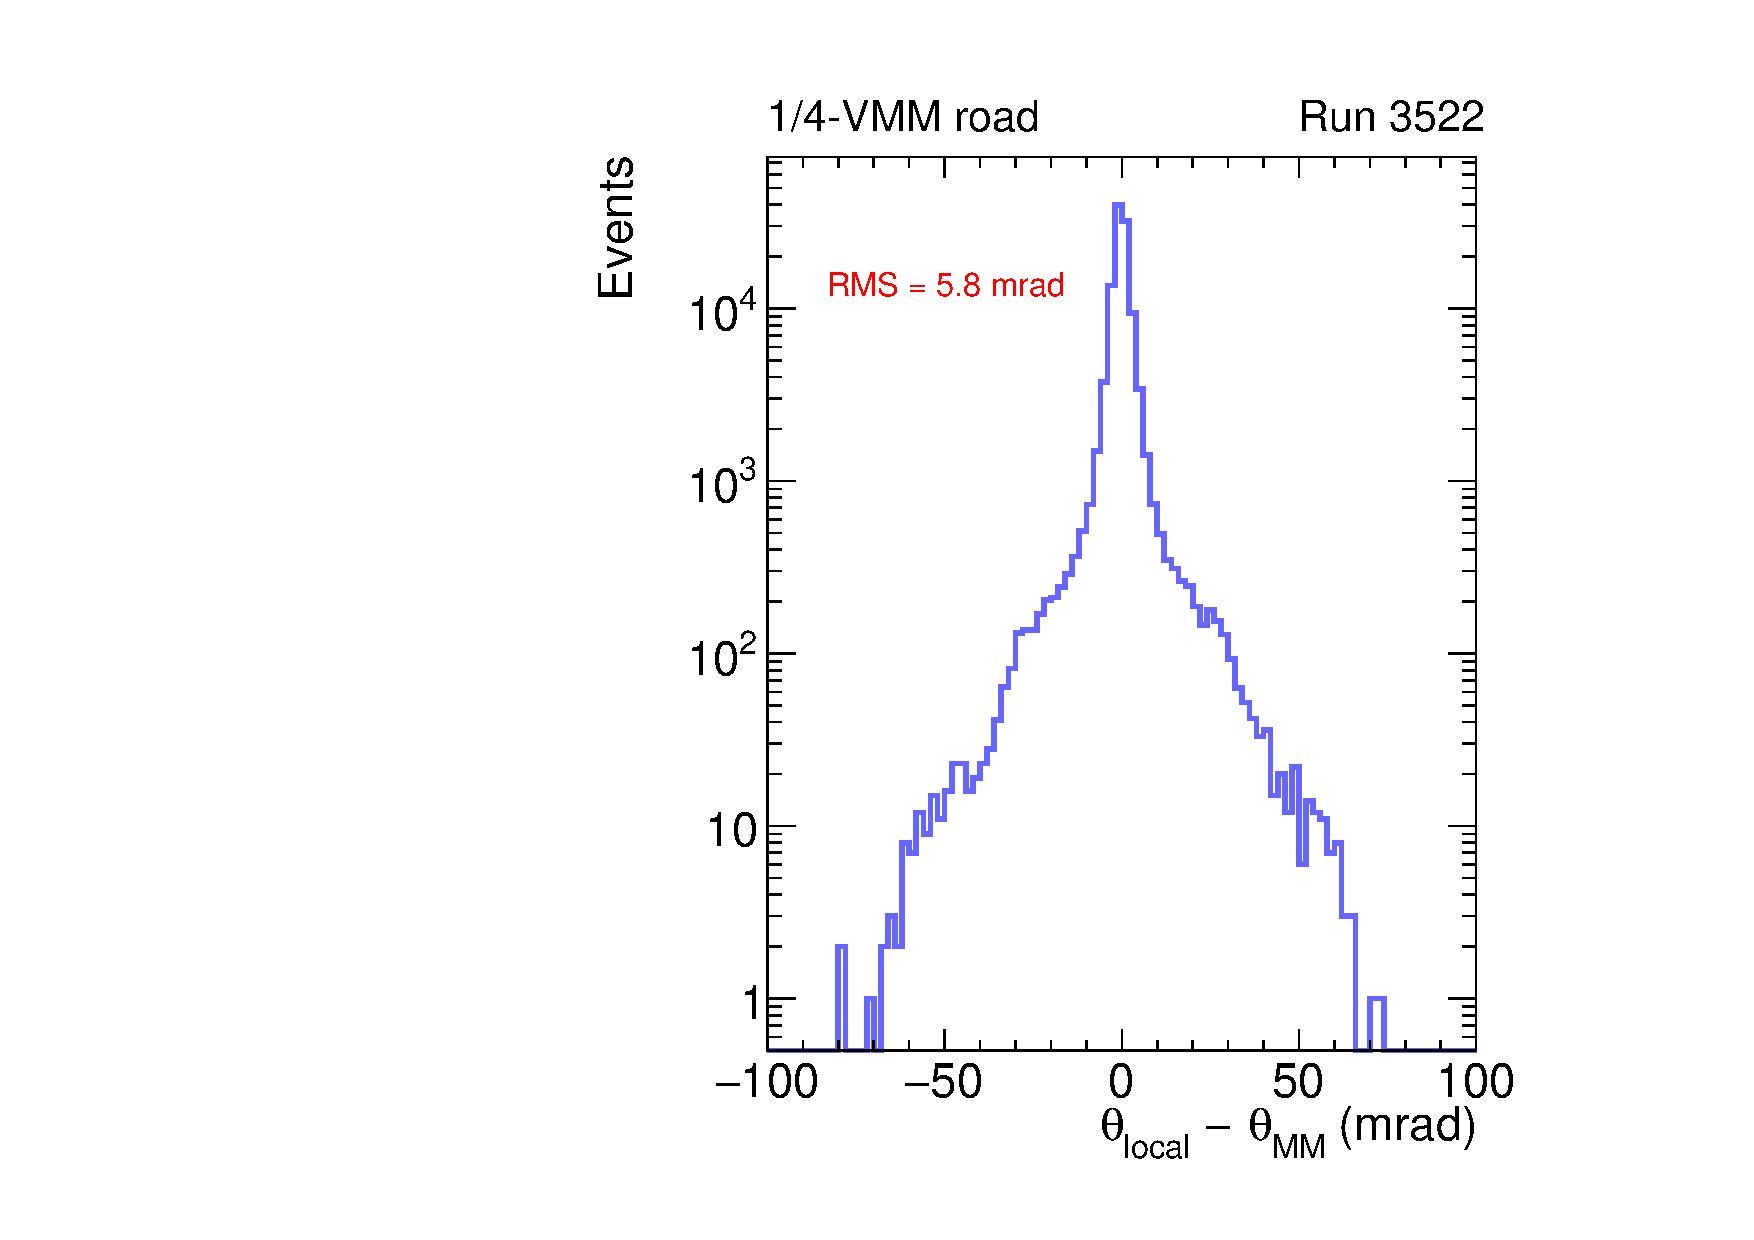
\includegraphics[width=0.4\textwidth]{figures/gbtanalysis3522/TP_angres.pdf}
  \end{center}
  \vspace{-10pt}
  \caption{The $\theta$ resolution of the MM TP relative to the full readout, using 1-VMM online roads (left) and 1/4-VMM offline roads (right). The tails of the resolution are greatly suppressed with smaller roads.}
  \label{fig:thetares}
\end{figure}

\begin{figure}[!htpb]
  \begin{center}
    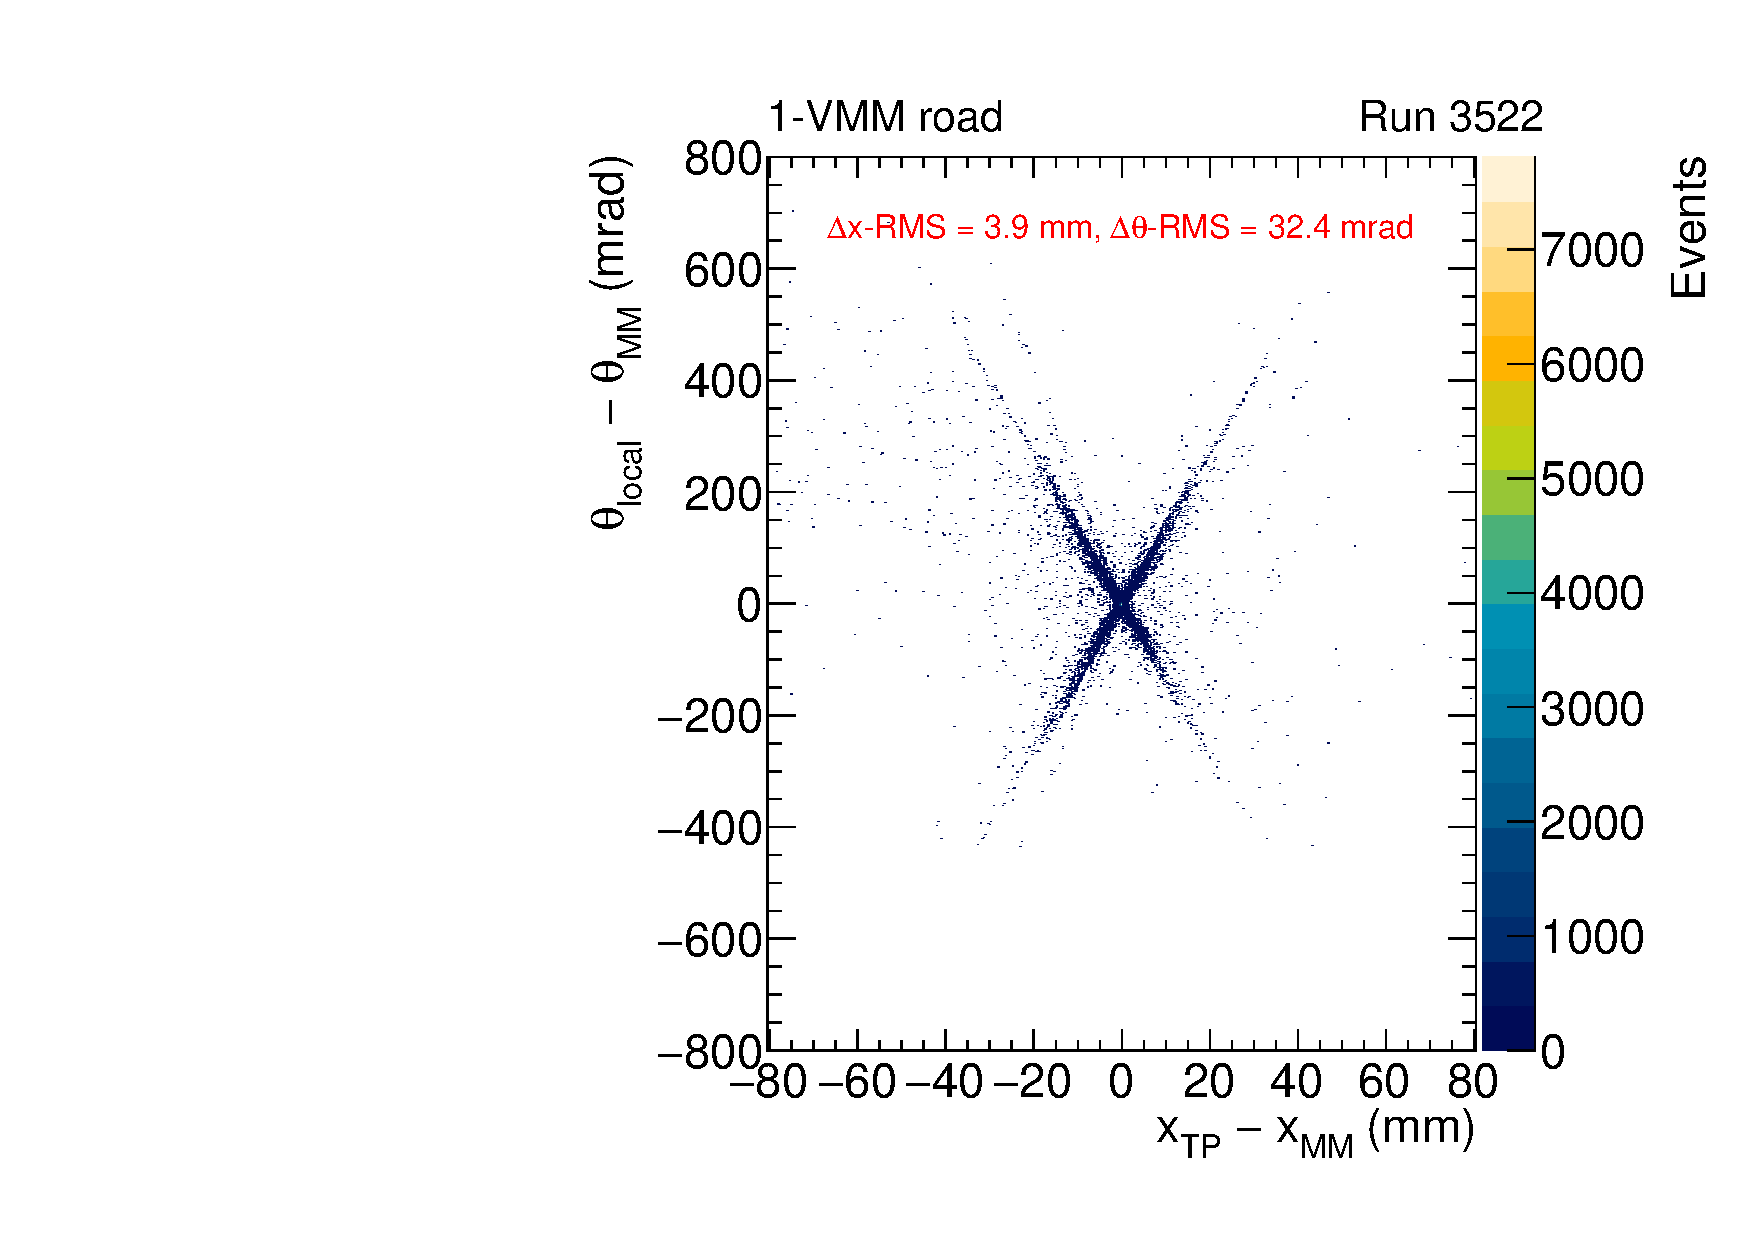
\includegraphics[width=0.4\textwidth]{figures/gbtanalysis3522/TP_xres_angres_full.pdf}
    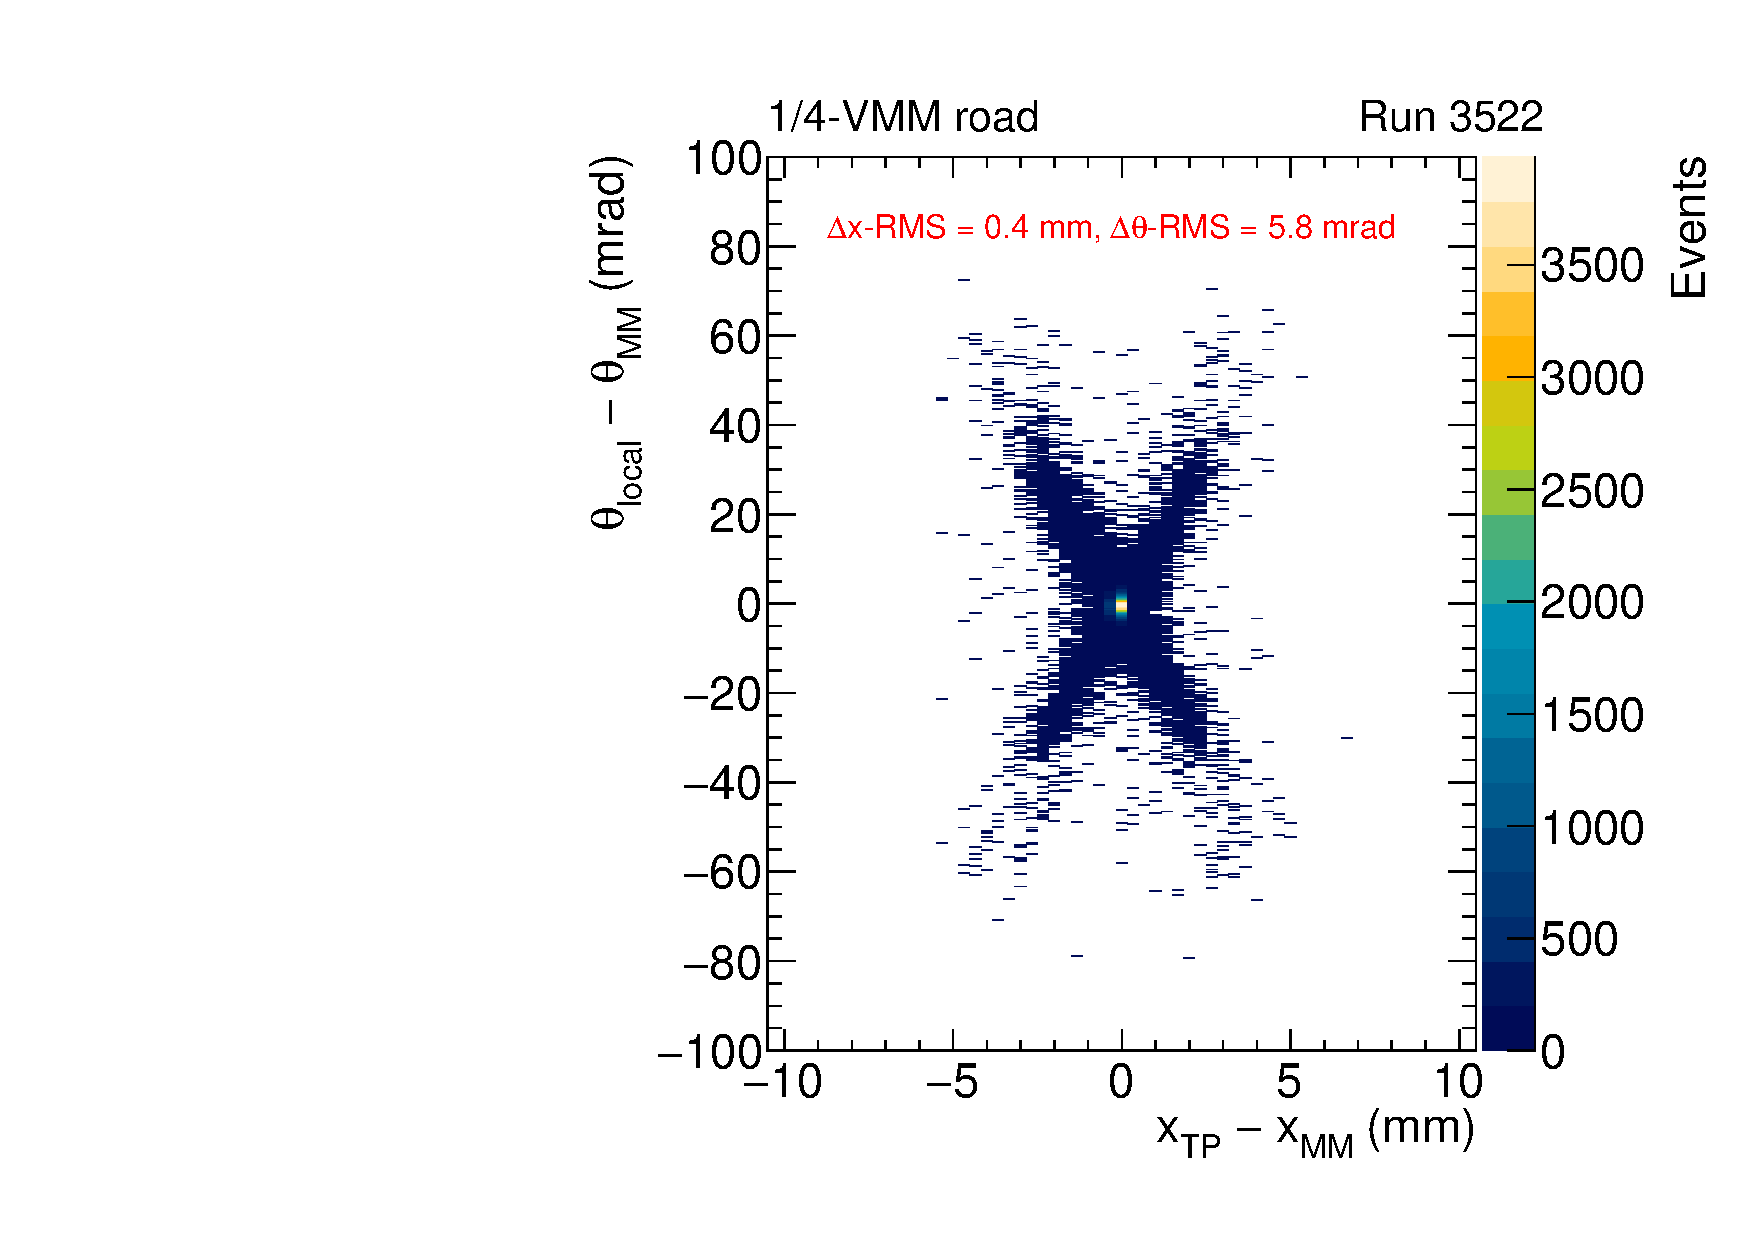
\includegraphics[width=0.4\textwidth]{figures/gbtanalysis3522/TP_xres_angres.pdf}
  \end{center}
  \vspace{-10pt}
  \caption{The $x$ and $\theta$ resolution of the MM TP relative to the full readout, using 1-VMM online roads (left) and 1/4-VMM offline roads (right). The tails of the resolution are greatly suppressed with smaller roads.}
  \label{fig:xthetares}
\end{figure}


\subsection{Time resolution}

\begin{figure}[!htpb]
  \begin{center}
    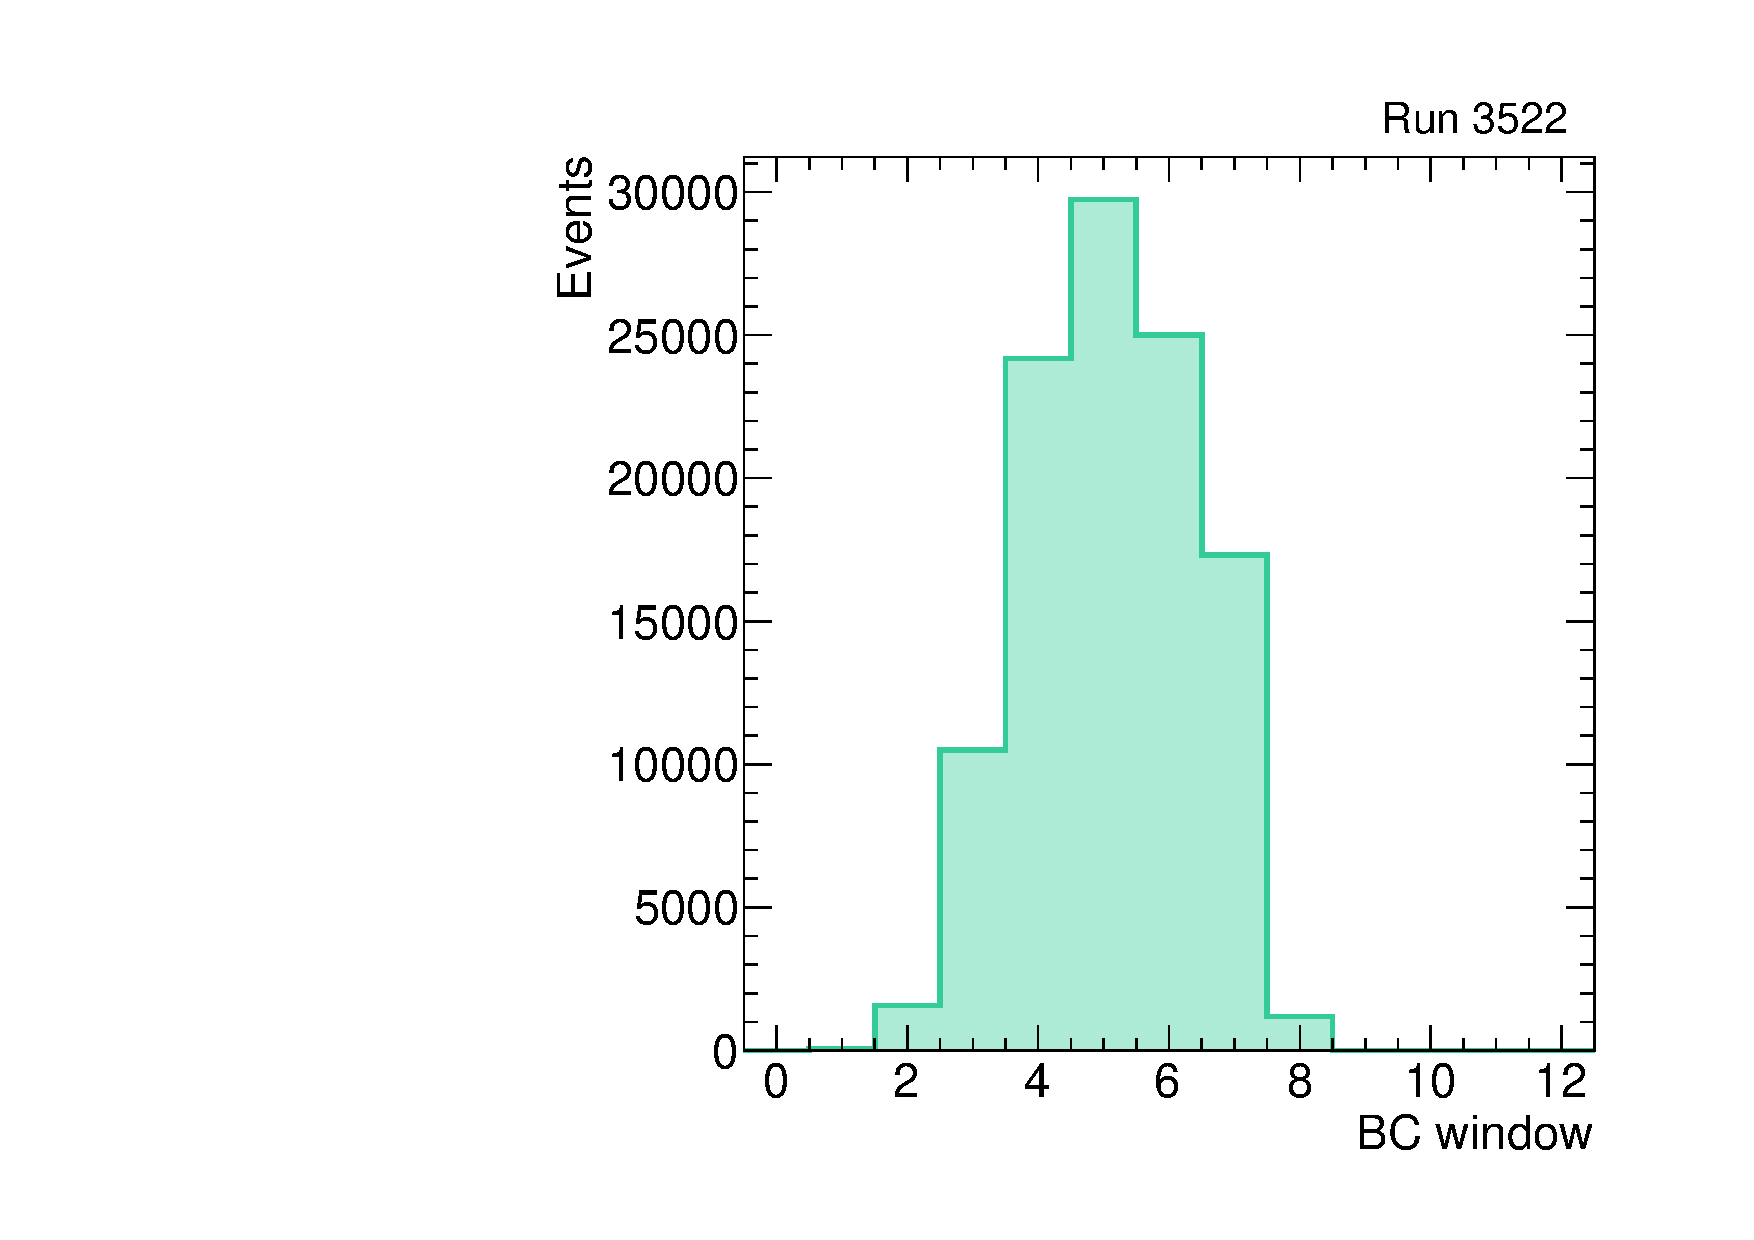
\includegraphics[width=0.4\textwidth]{figures/gbtanalysis3522/artwin_lin.pdf}
    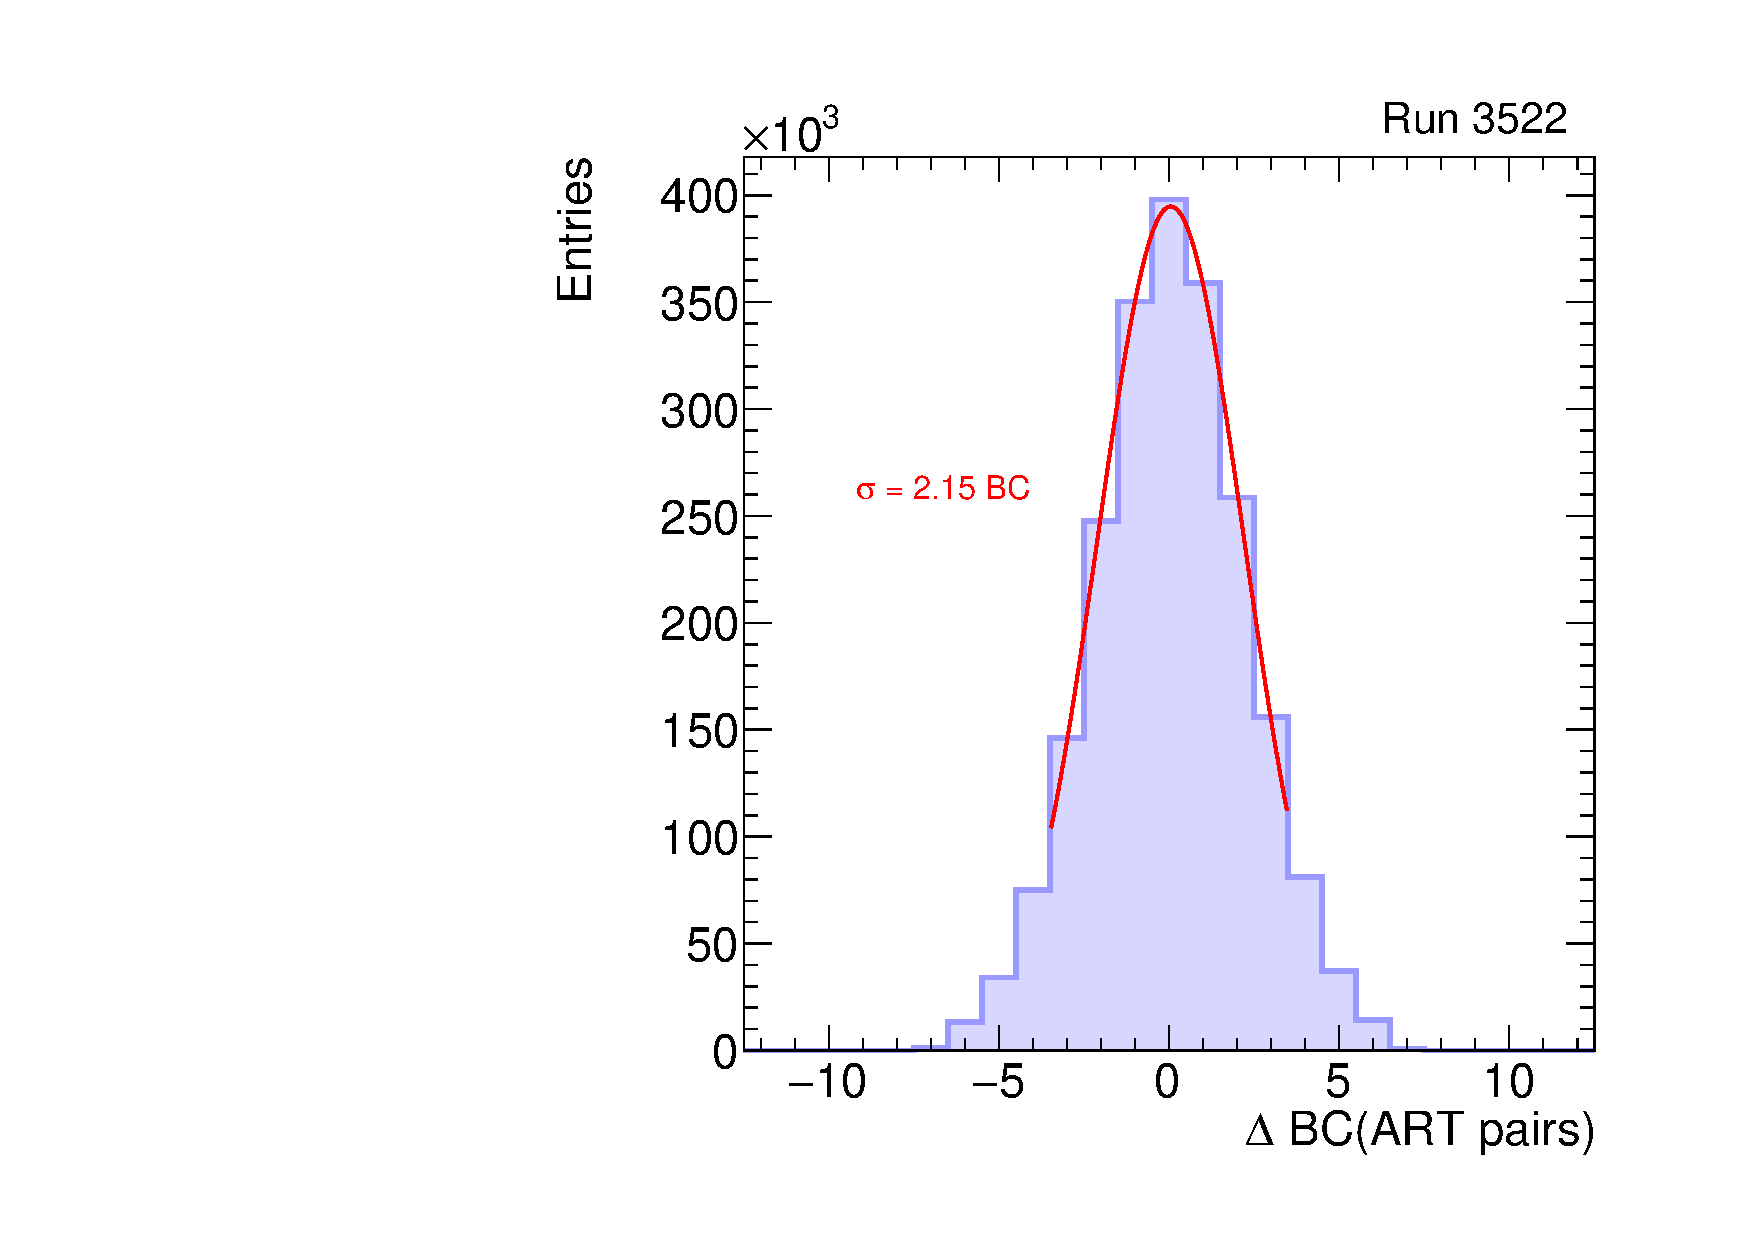
\includegraphics[width=0.4\textwidth]{figures/gbtanalysis3522/artrpairs_lin.pdf}
  \end{center}
  \vspace{-10pt}
  \caption{The time window required to record all hits in a trigger (left) and the $\Delta\text{BC}$ of all pairs of hits in a trigger (right). A gaussian fit is overlaid on the distribution of $\Delta\text{BC}$ and describes the data well.}
  \label{fig:time}
\end{figure}

\begin{figure}[!htpb]
  \begin{center}
    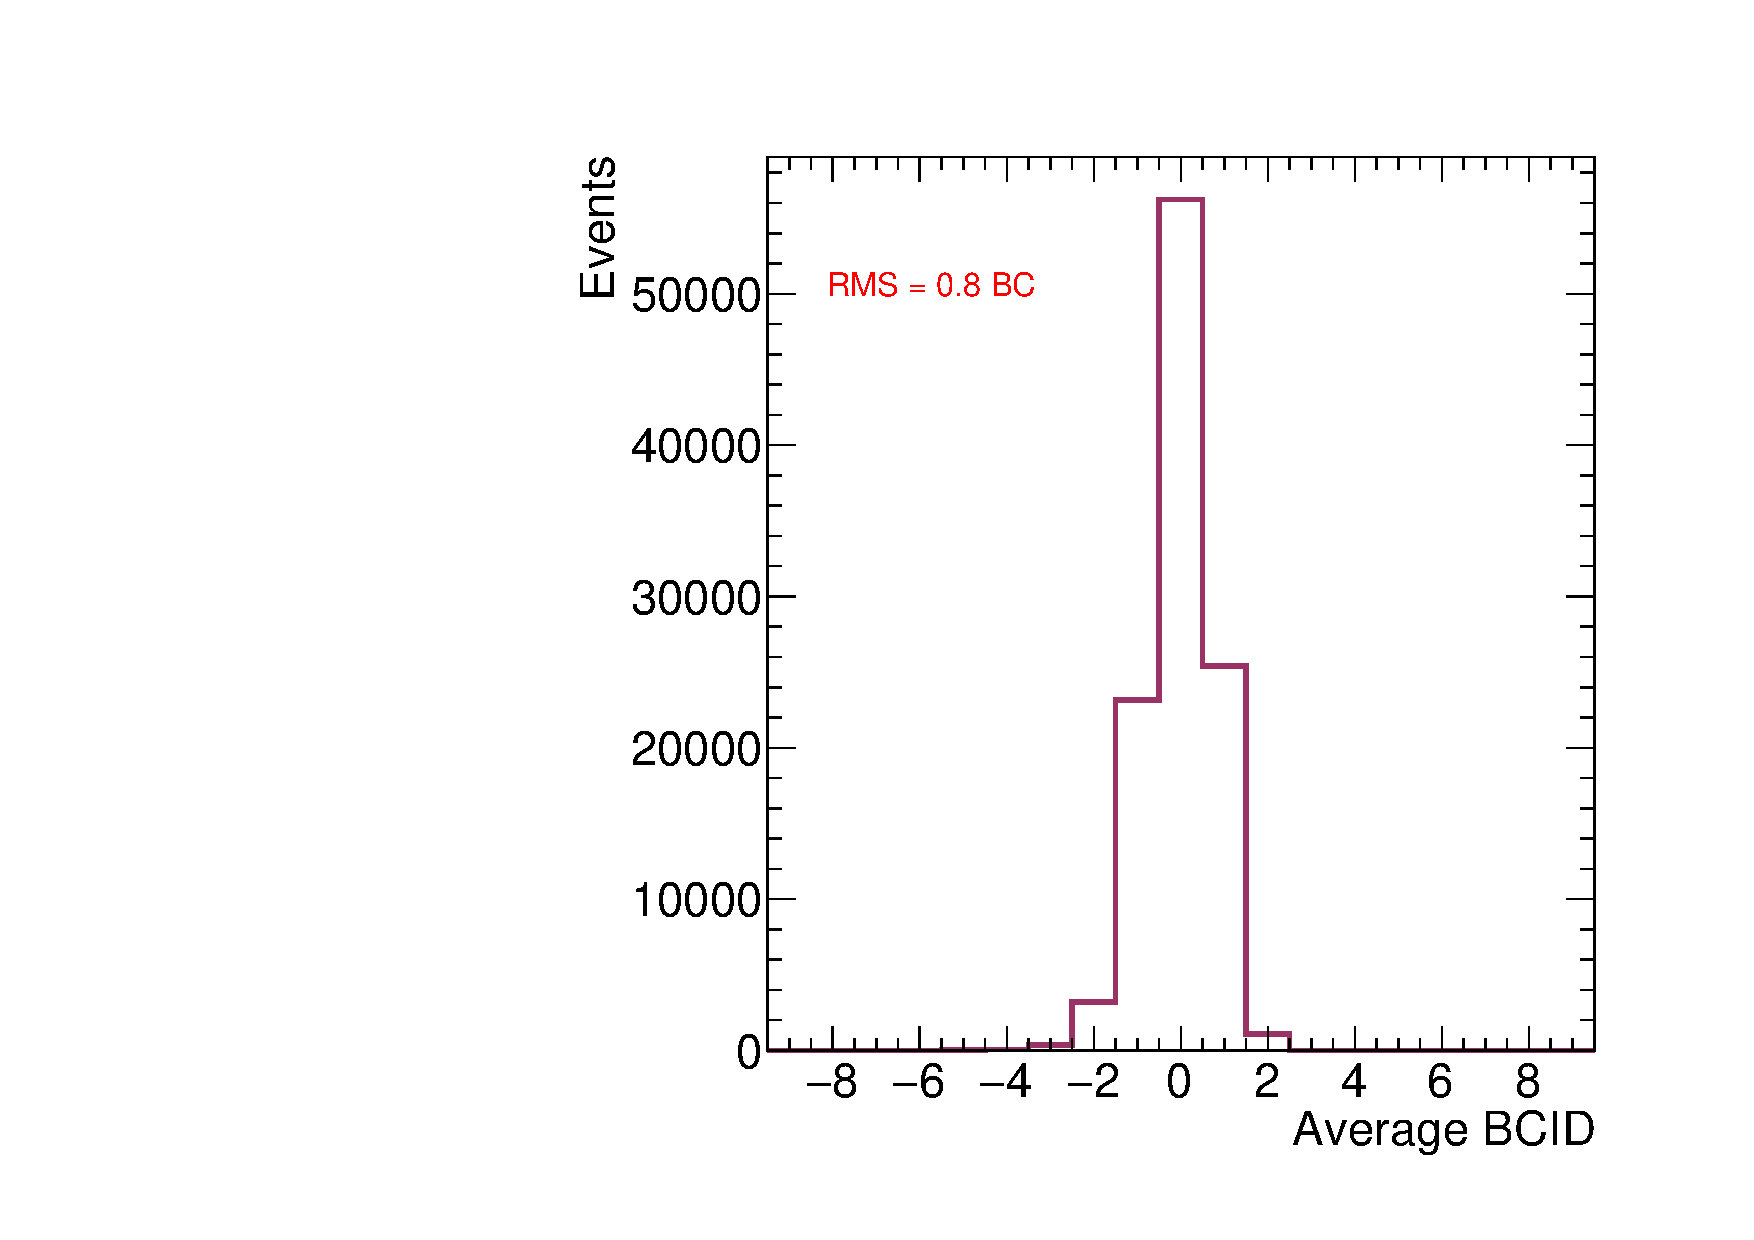
\includegraphics[width=0.4\textwidth]{figures/gbtanalysis3522/avg_BCID.pdf}
    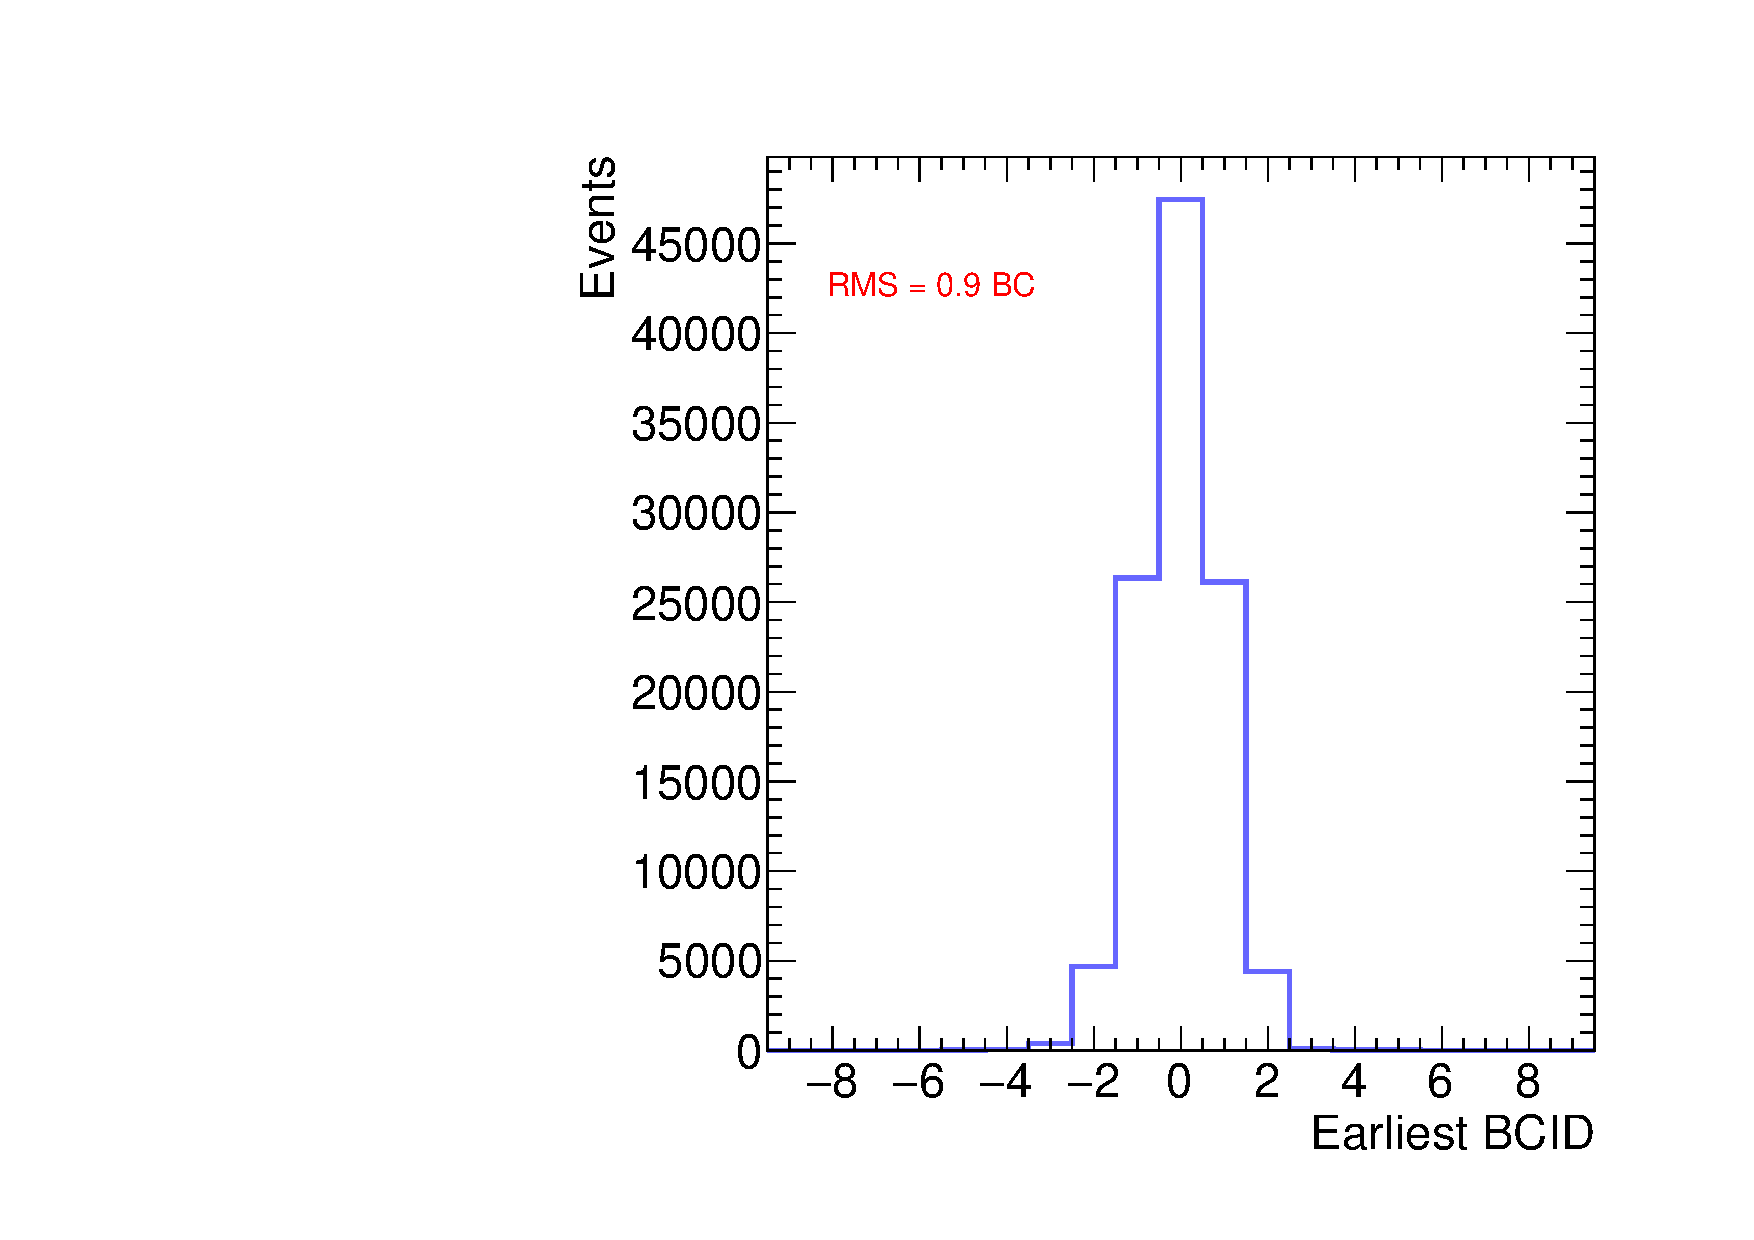
\includegraphics[width=0.4\textwidth]{figures/gbtanalysis3522/earliest_BCID.pdf}
  \end{center}
  \vspace{-10pt}
  \caption{The time resolution of the MM TP relative to the scintillator. The BCID of the trigger can be defined as the average BCID of the ART hits (left) or the earliest BCID (right). Choosing the average BCID has better resolution than choosing the earliest.}
  \label{fig:timeres}
\end{figure}

\subsection{Integration time}
\label{sec:perf-integ}

\begin{figure}[!htpb]
  \begin{center}
    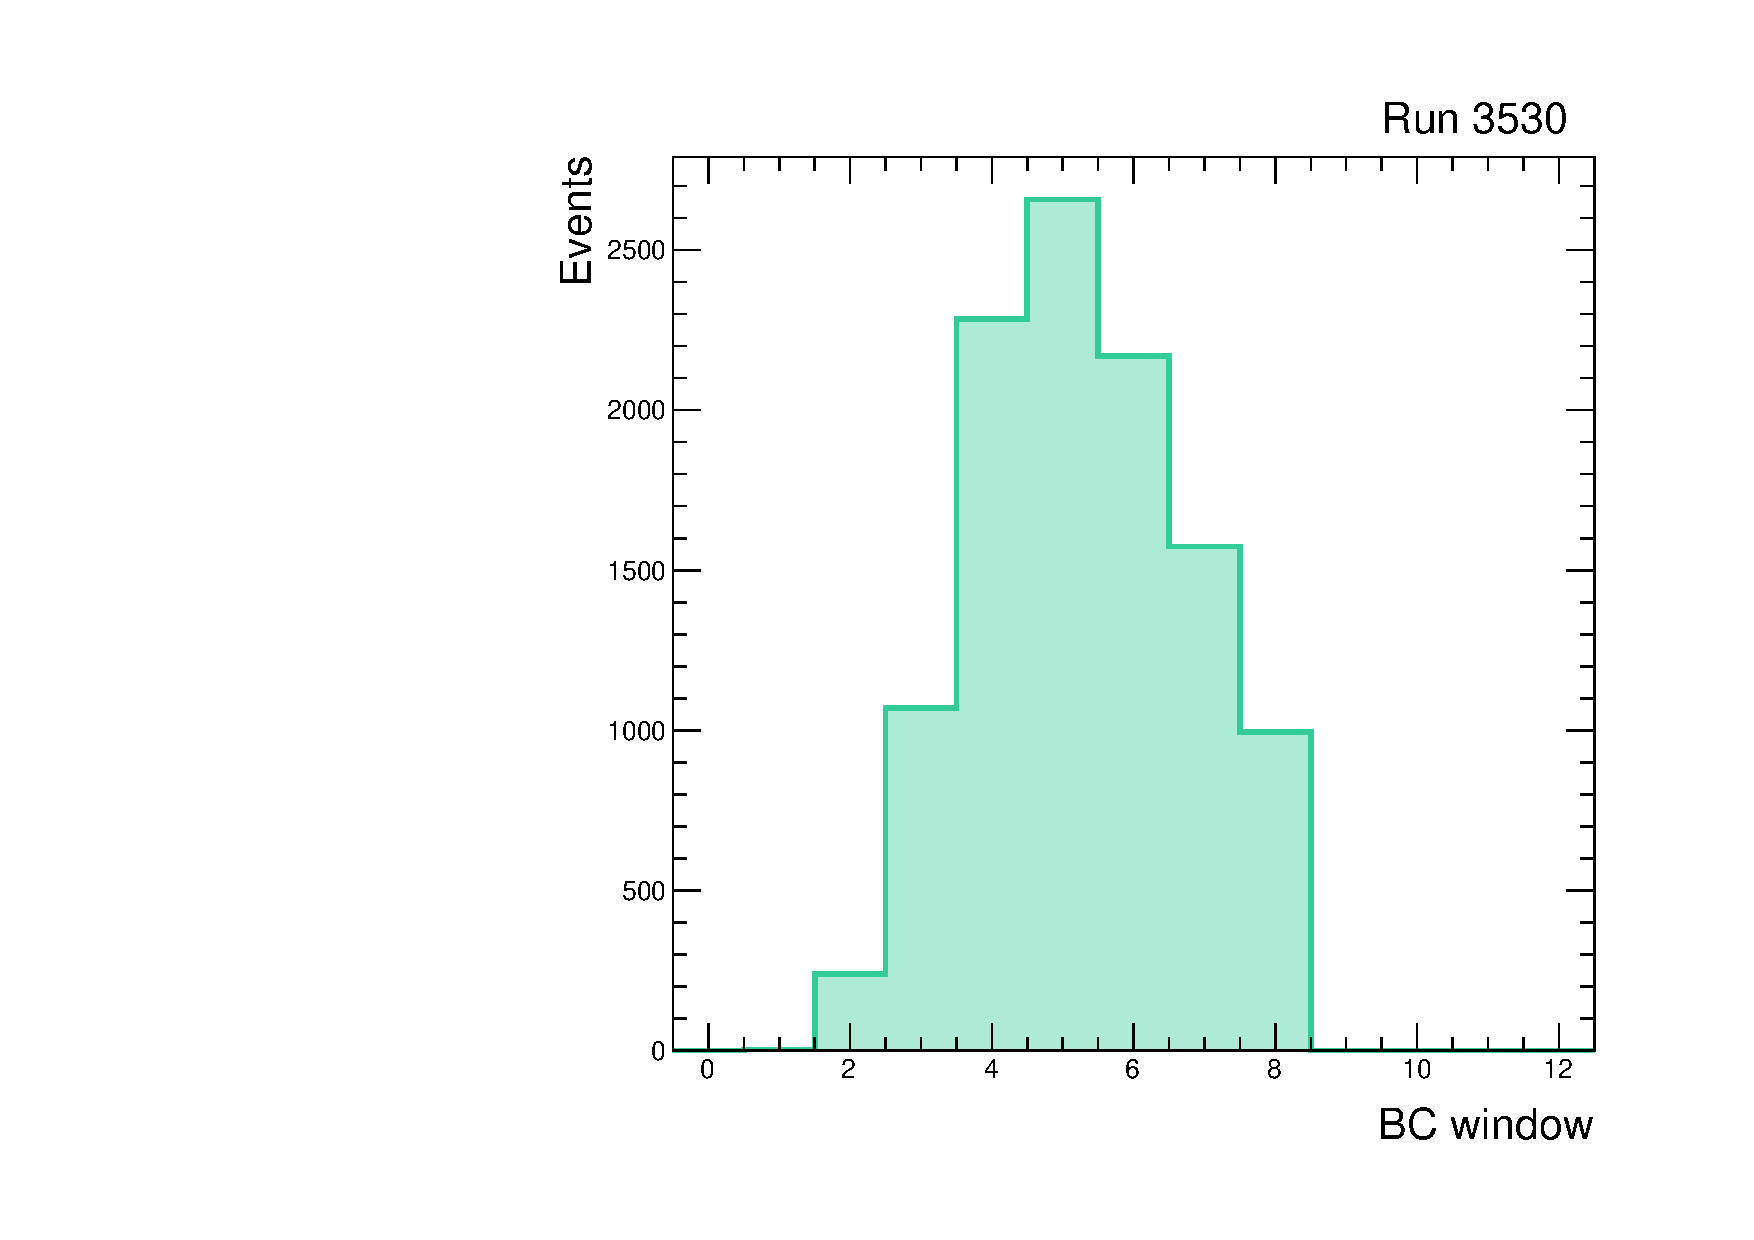
\includegraphics[width=0.3\textwidth]{figures/gbtanalysis3530/artwin_lin.pdf}
    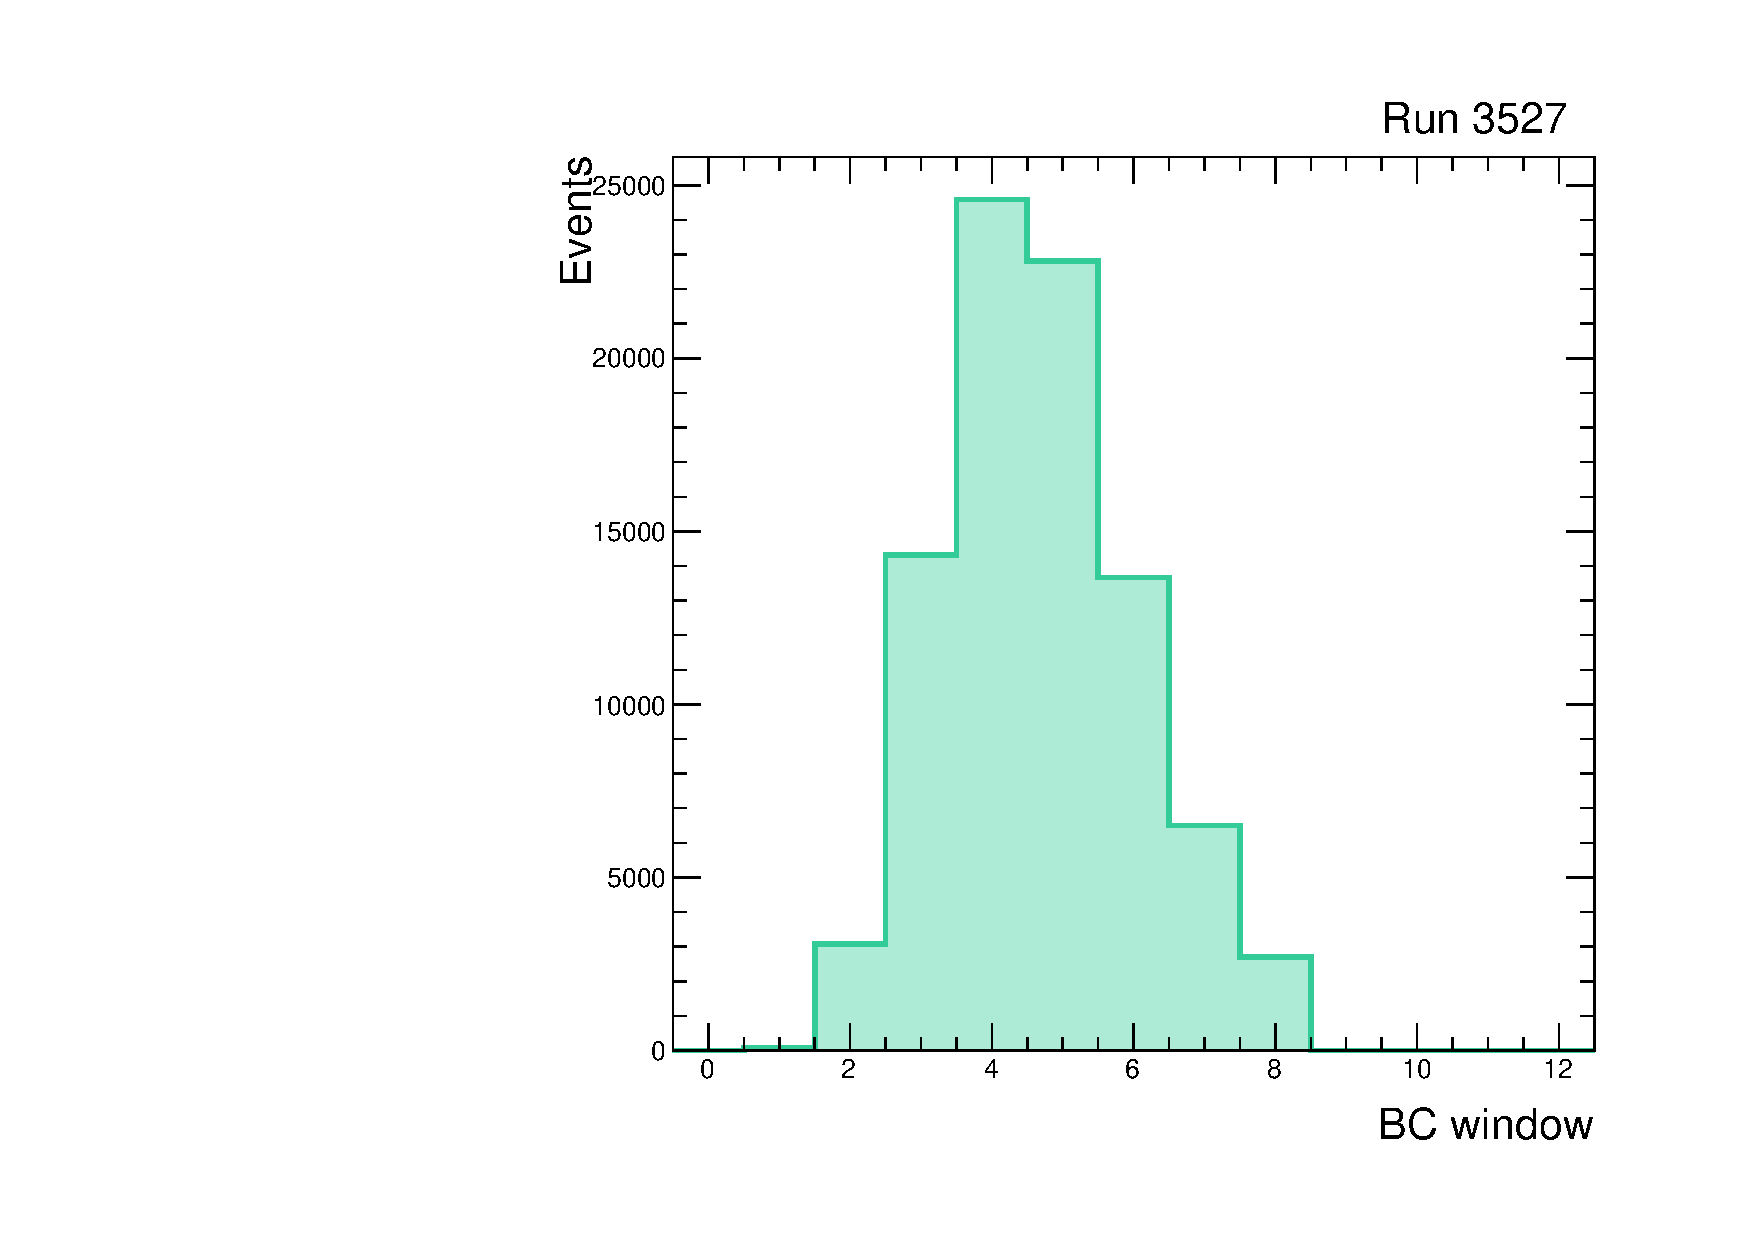
\includegraphics[width=0.3\textwidth]{figures/gbtanalysis3527/artwin_lin.pdf}
    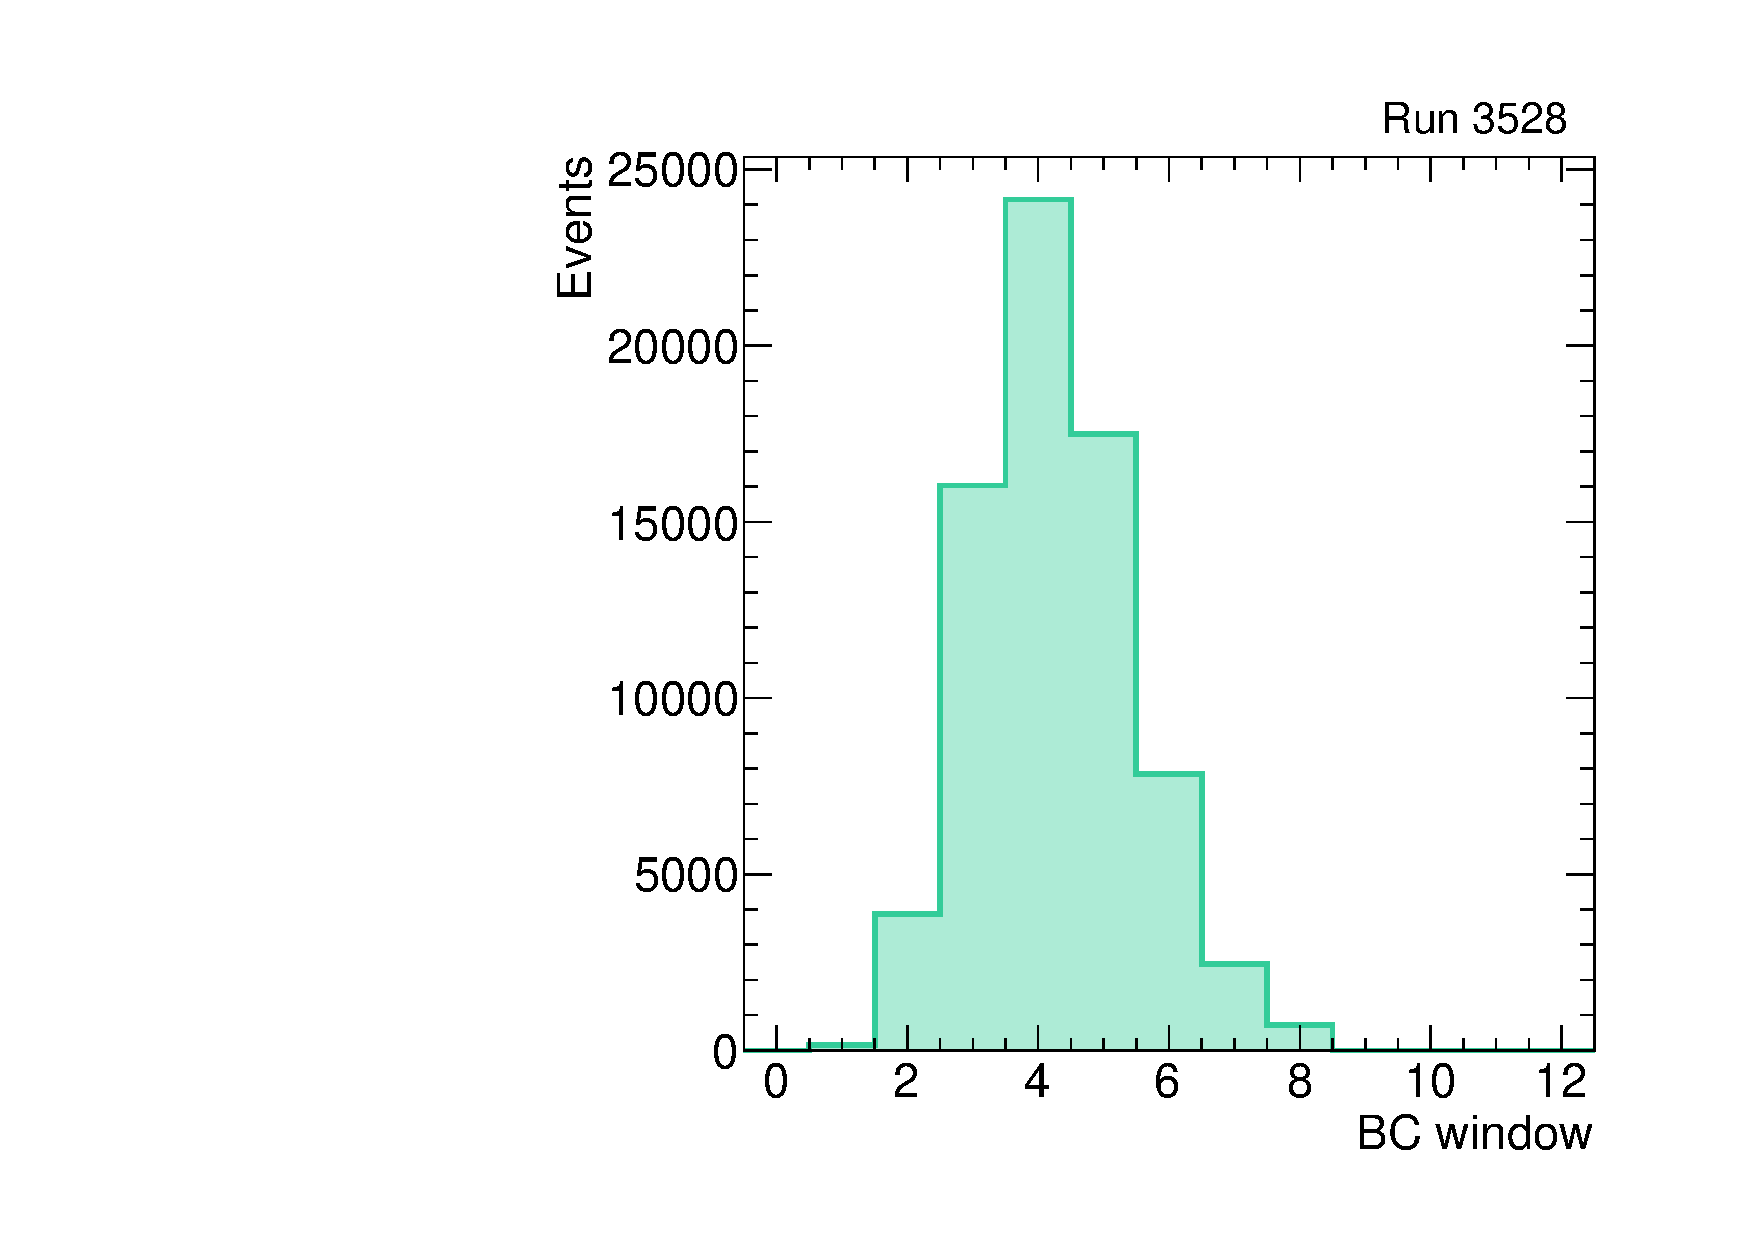
\includegraphics[width=0.3\textwidth]{figures/gbtanalysis3528/artwin_lin.pdf}
  \end{center}
  \vspace{-10pt}
  \caption{The time window required to record all hits in a trigger for data collected with 200 ns (left), 100 ns (middle), and 50 ns (right) integration time in the VMM. The window decreases as the integration time decreases.}
  \label{fig:integ_window}
\end{figure}

\begin{figure}[!htpb]
  \begin{center}
    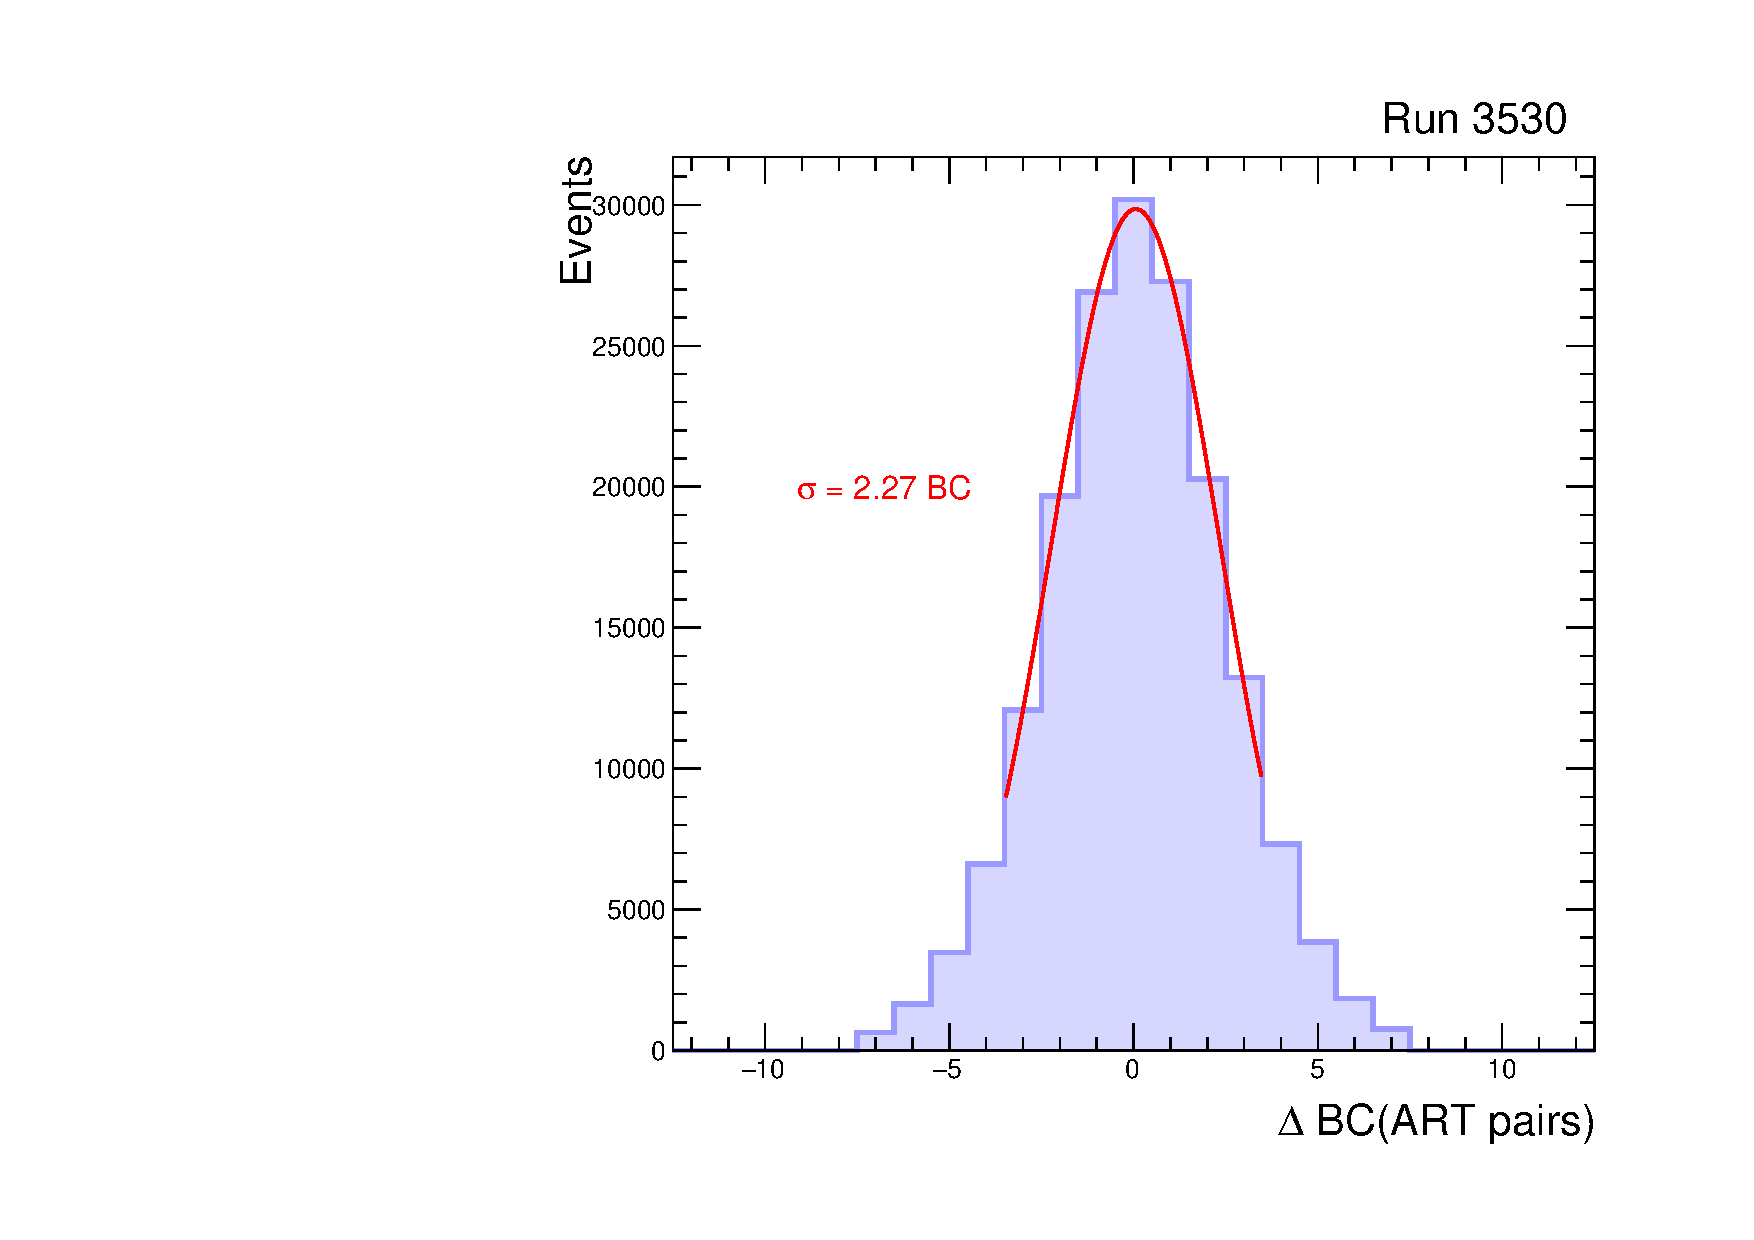
\includegraphics[width=0.3\textwidth]{figures/gbtanalysis3530/artrpairs_lin.pdf}
    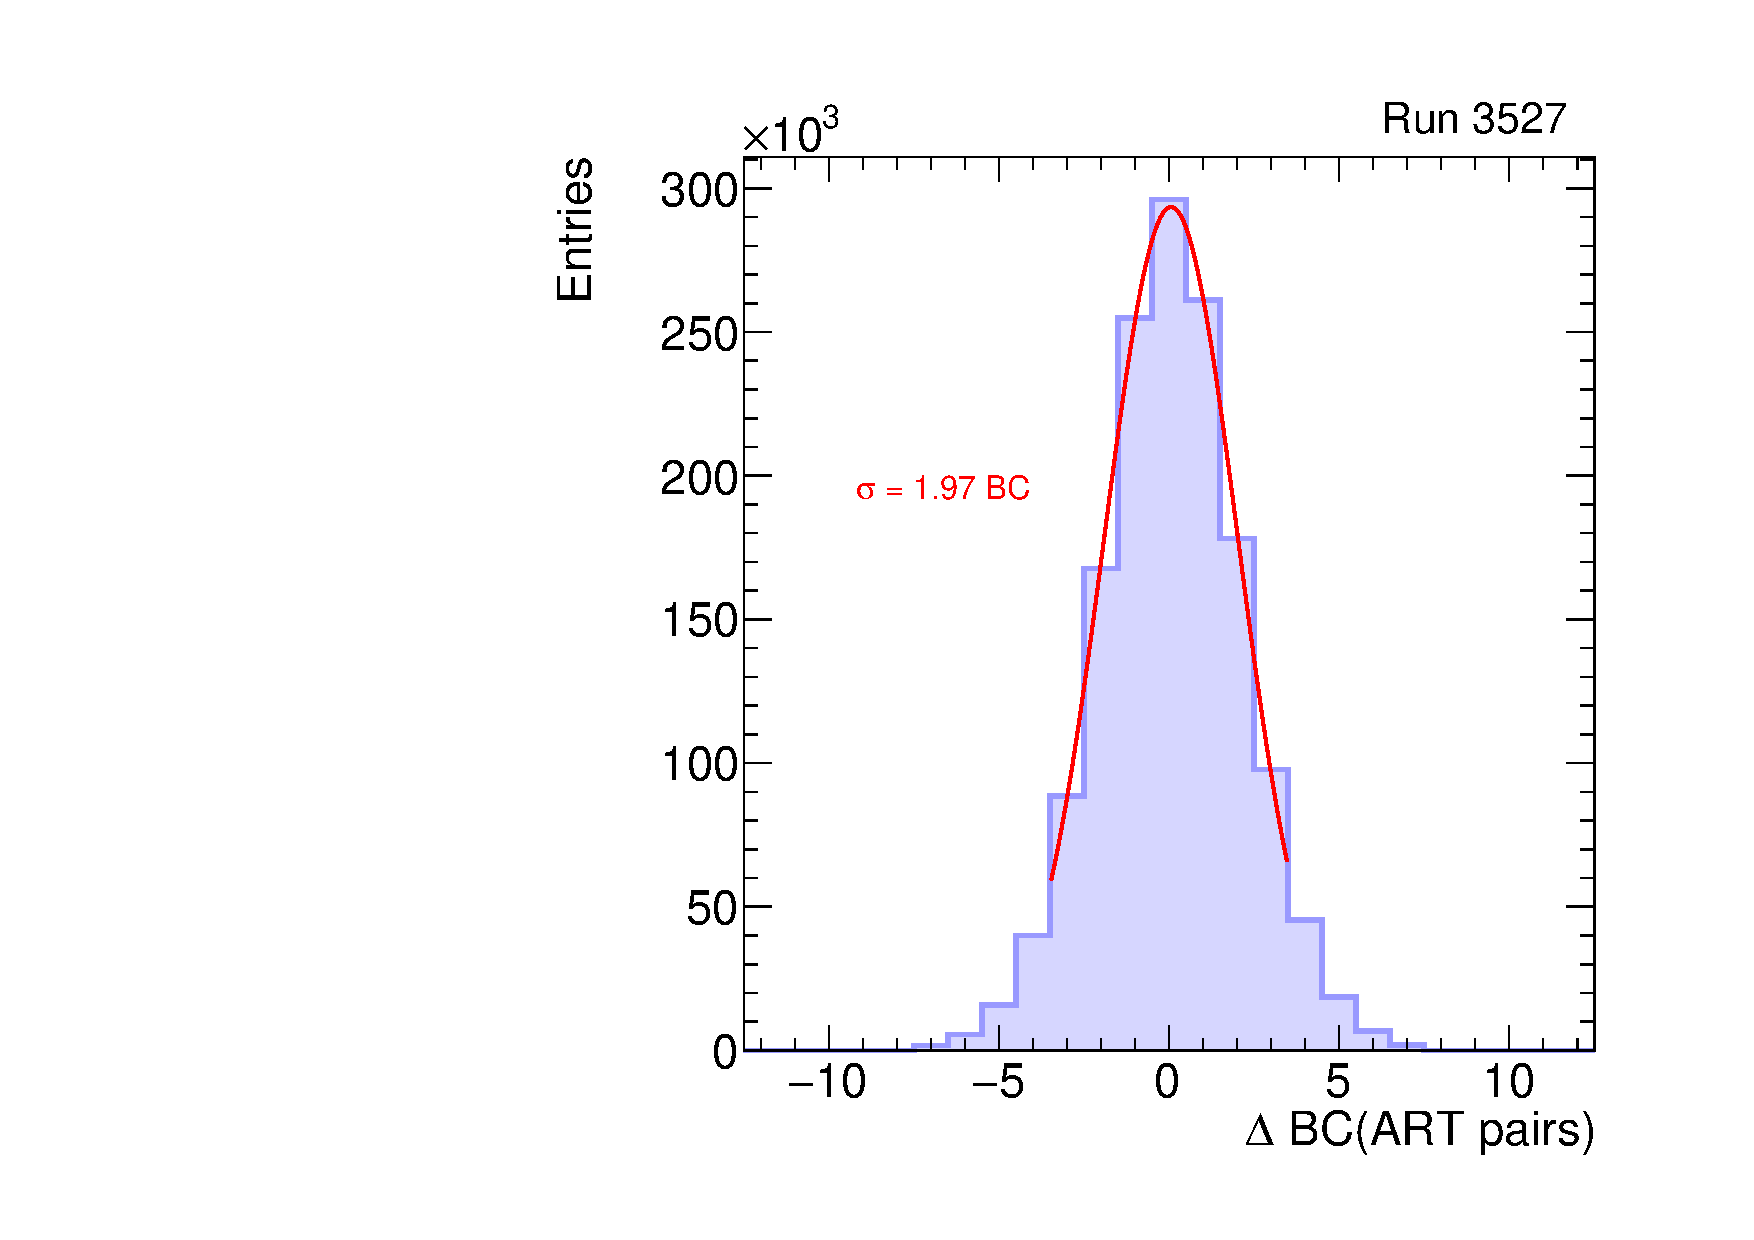
\includegraphics[width=0.3\textwidth]{figures/gbtanalysis3527/artrpairs_lin.pdf}
    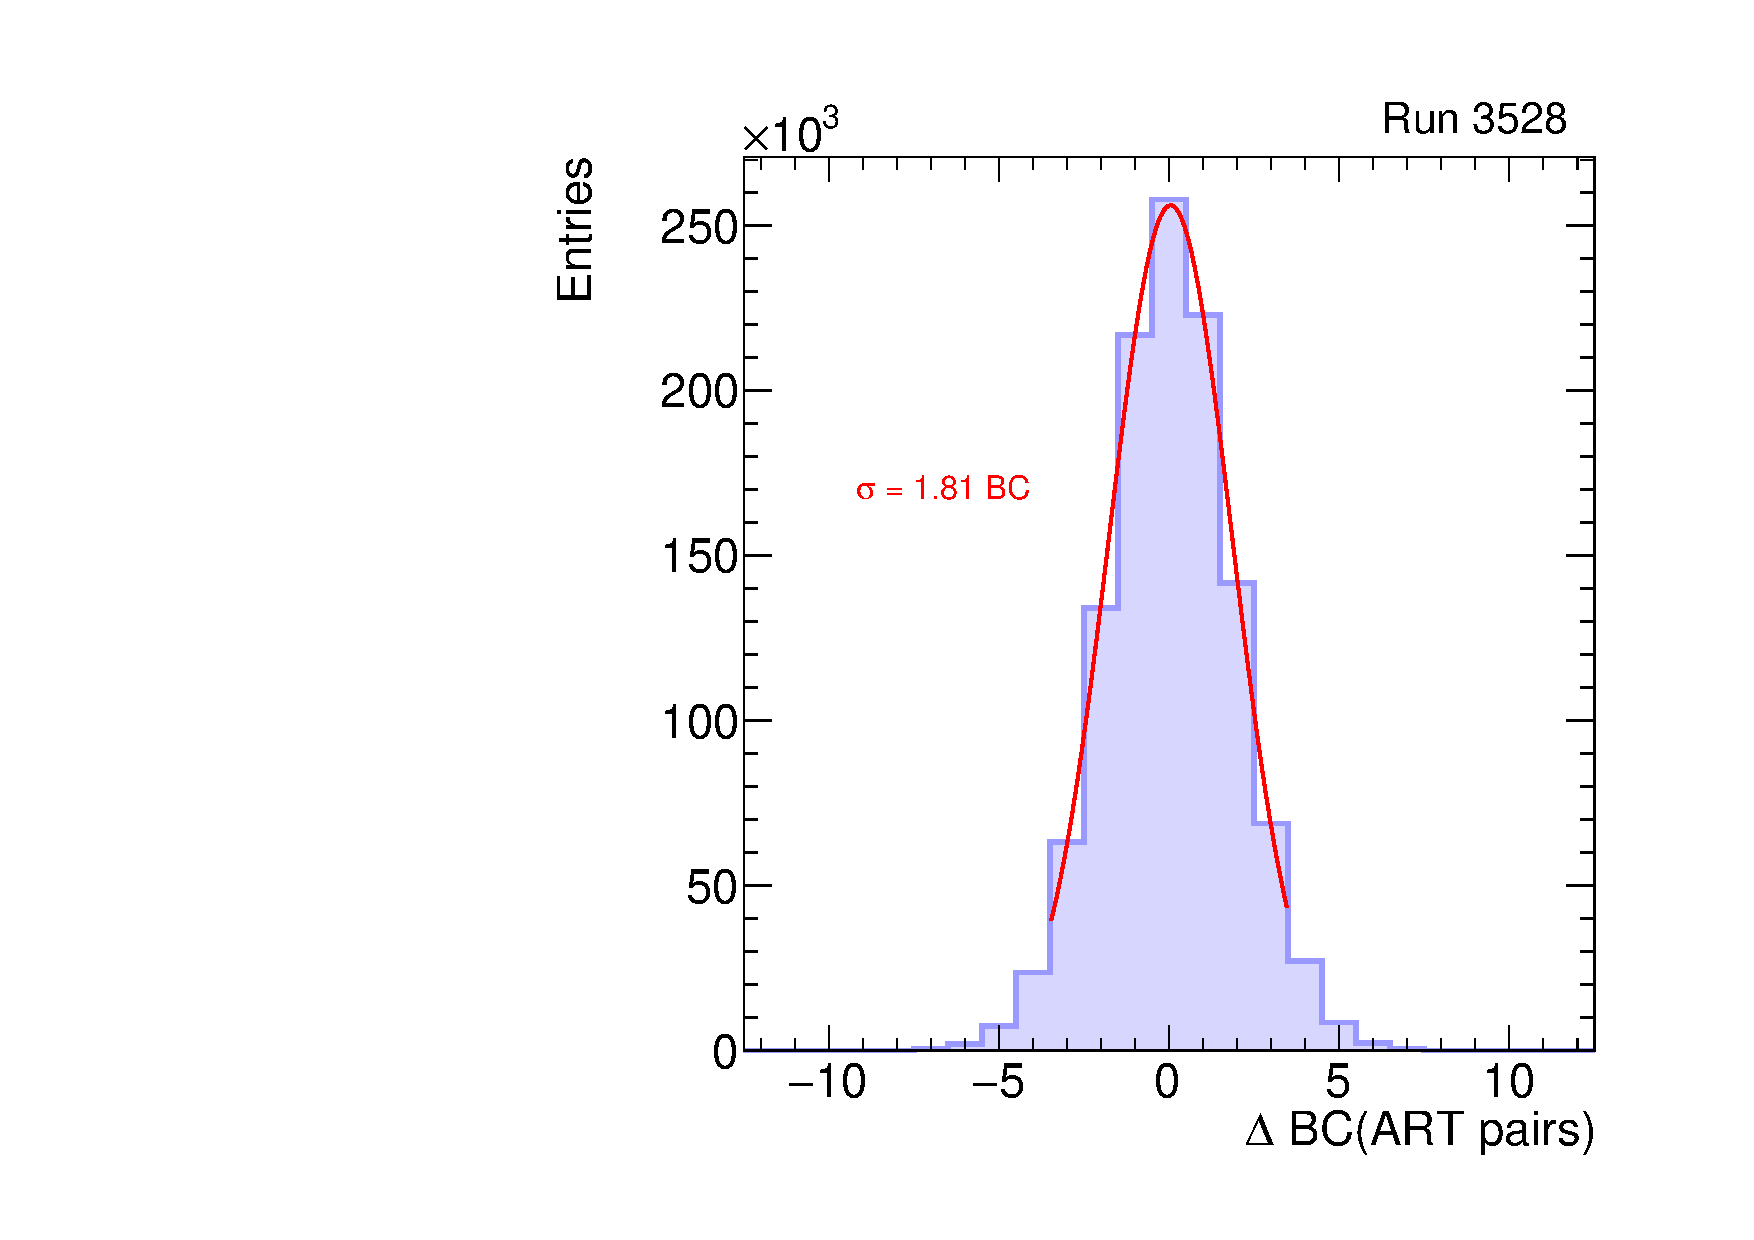
\includegraphics[width=0.3\textwidth]{figures/gbtanalysis3528/artrpairs_lin.pdf}
  \end{center}
  \vspace{-10pt}
  \caption{The $\Delta\text{BC}$ of all pairs of hits in a trigger for data collected with 200 ns (left), 100 ns (middle), and 50 ns (right) integration time in the VMM. The distribution is narrower as the integration time decreases.}
  \label{fig:integ_pairs}
\end{figure}

\begin{figure}[!htpb]
  \begin{center}
    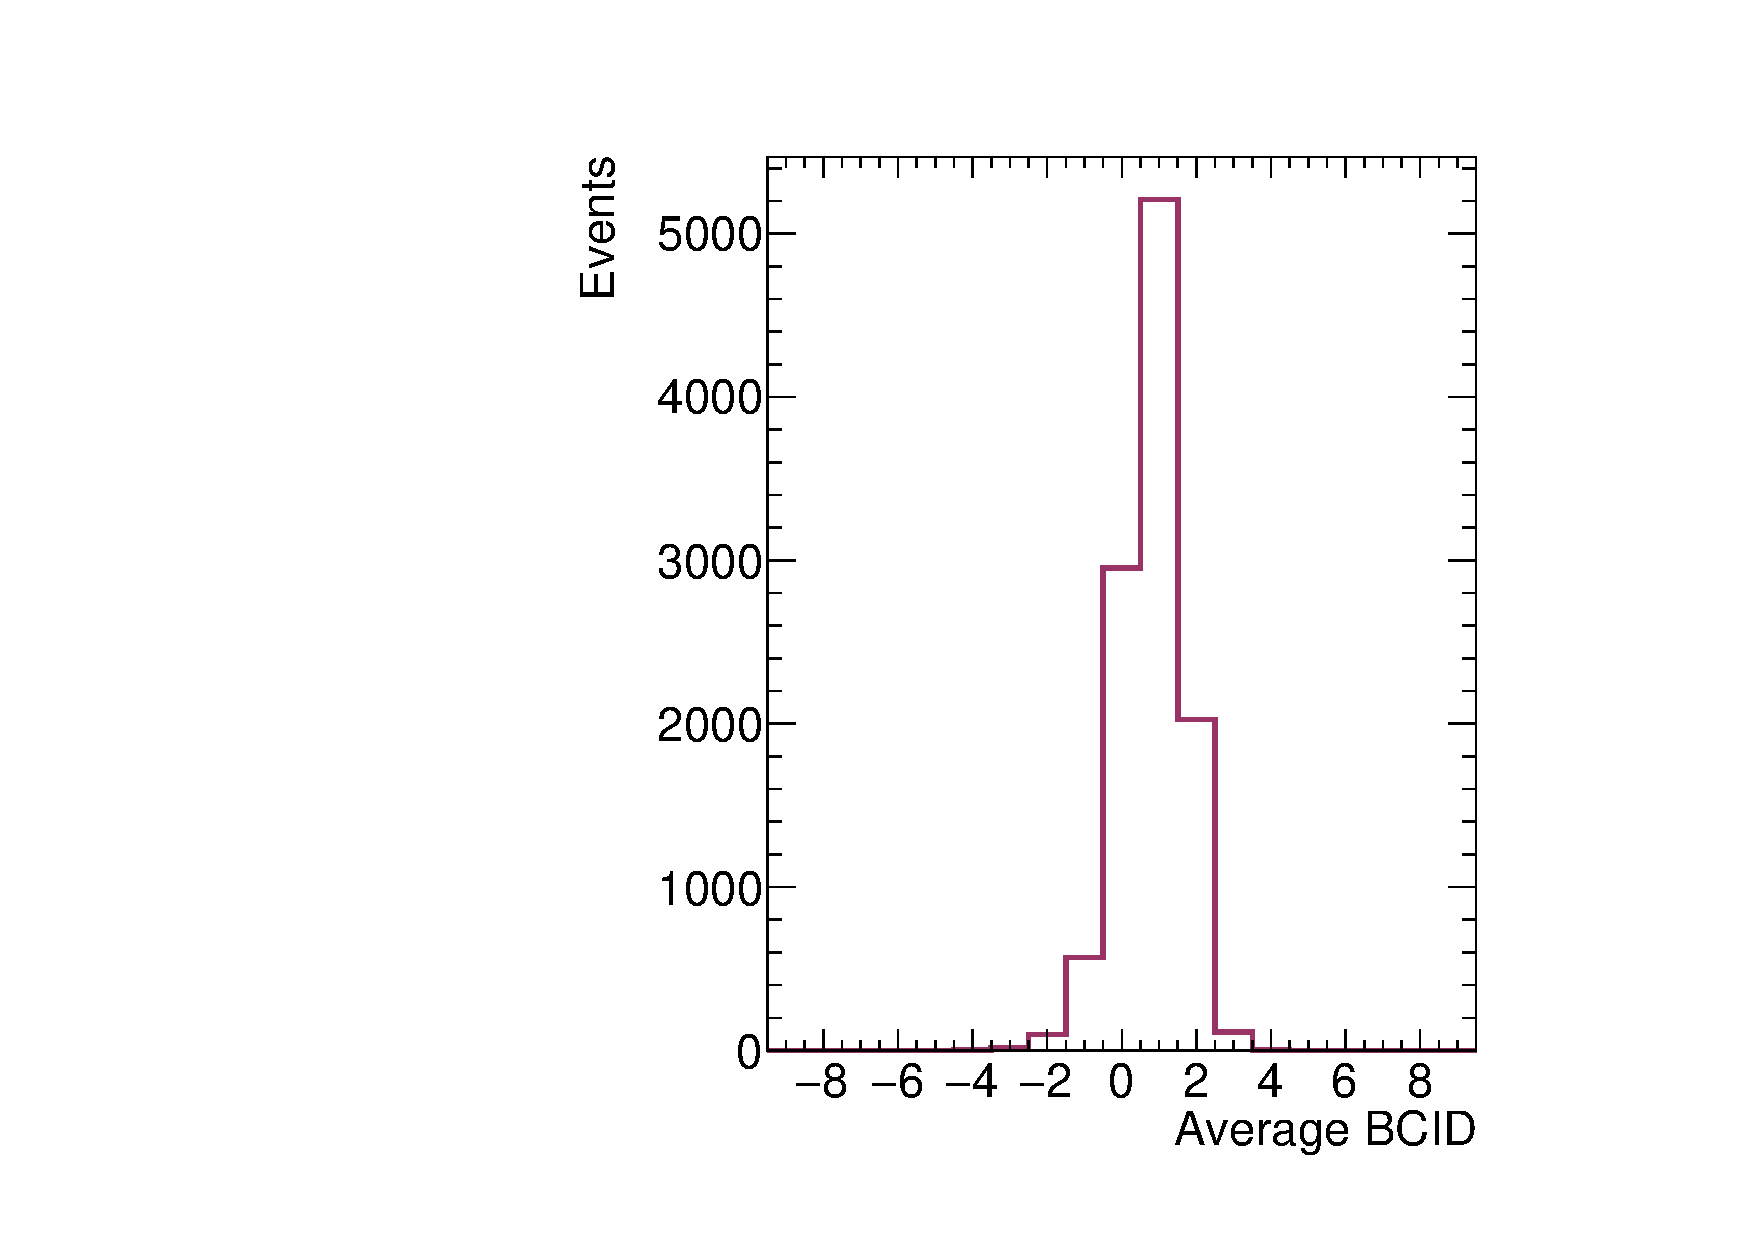
\includegraphics[width=0.3\textwidth]{figures/gbtanalysis3530/avg_BCID.pdf}
    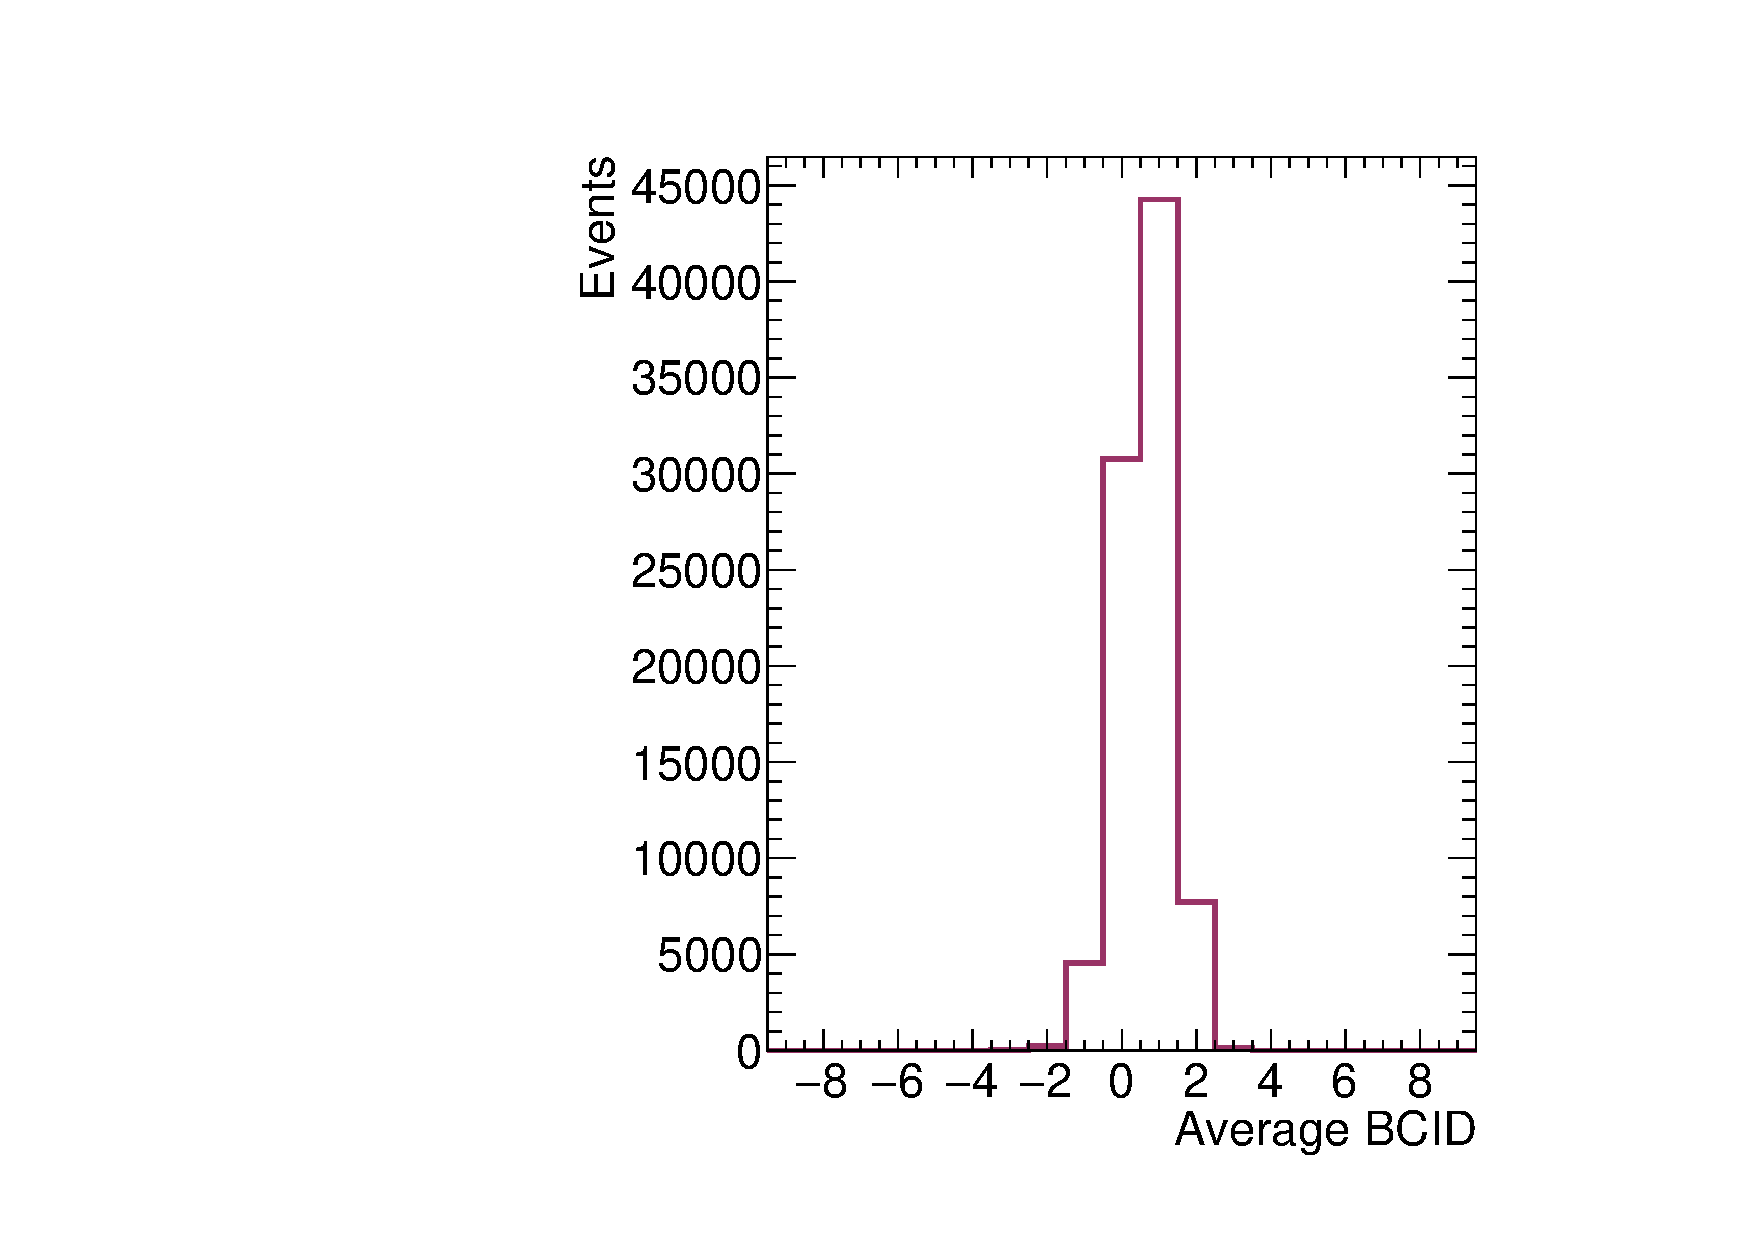
\includegraphics[width=0.3\textwidth]{figures/gbtanalysis3527/avg_BCID.pdf}
    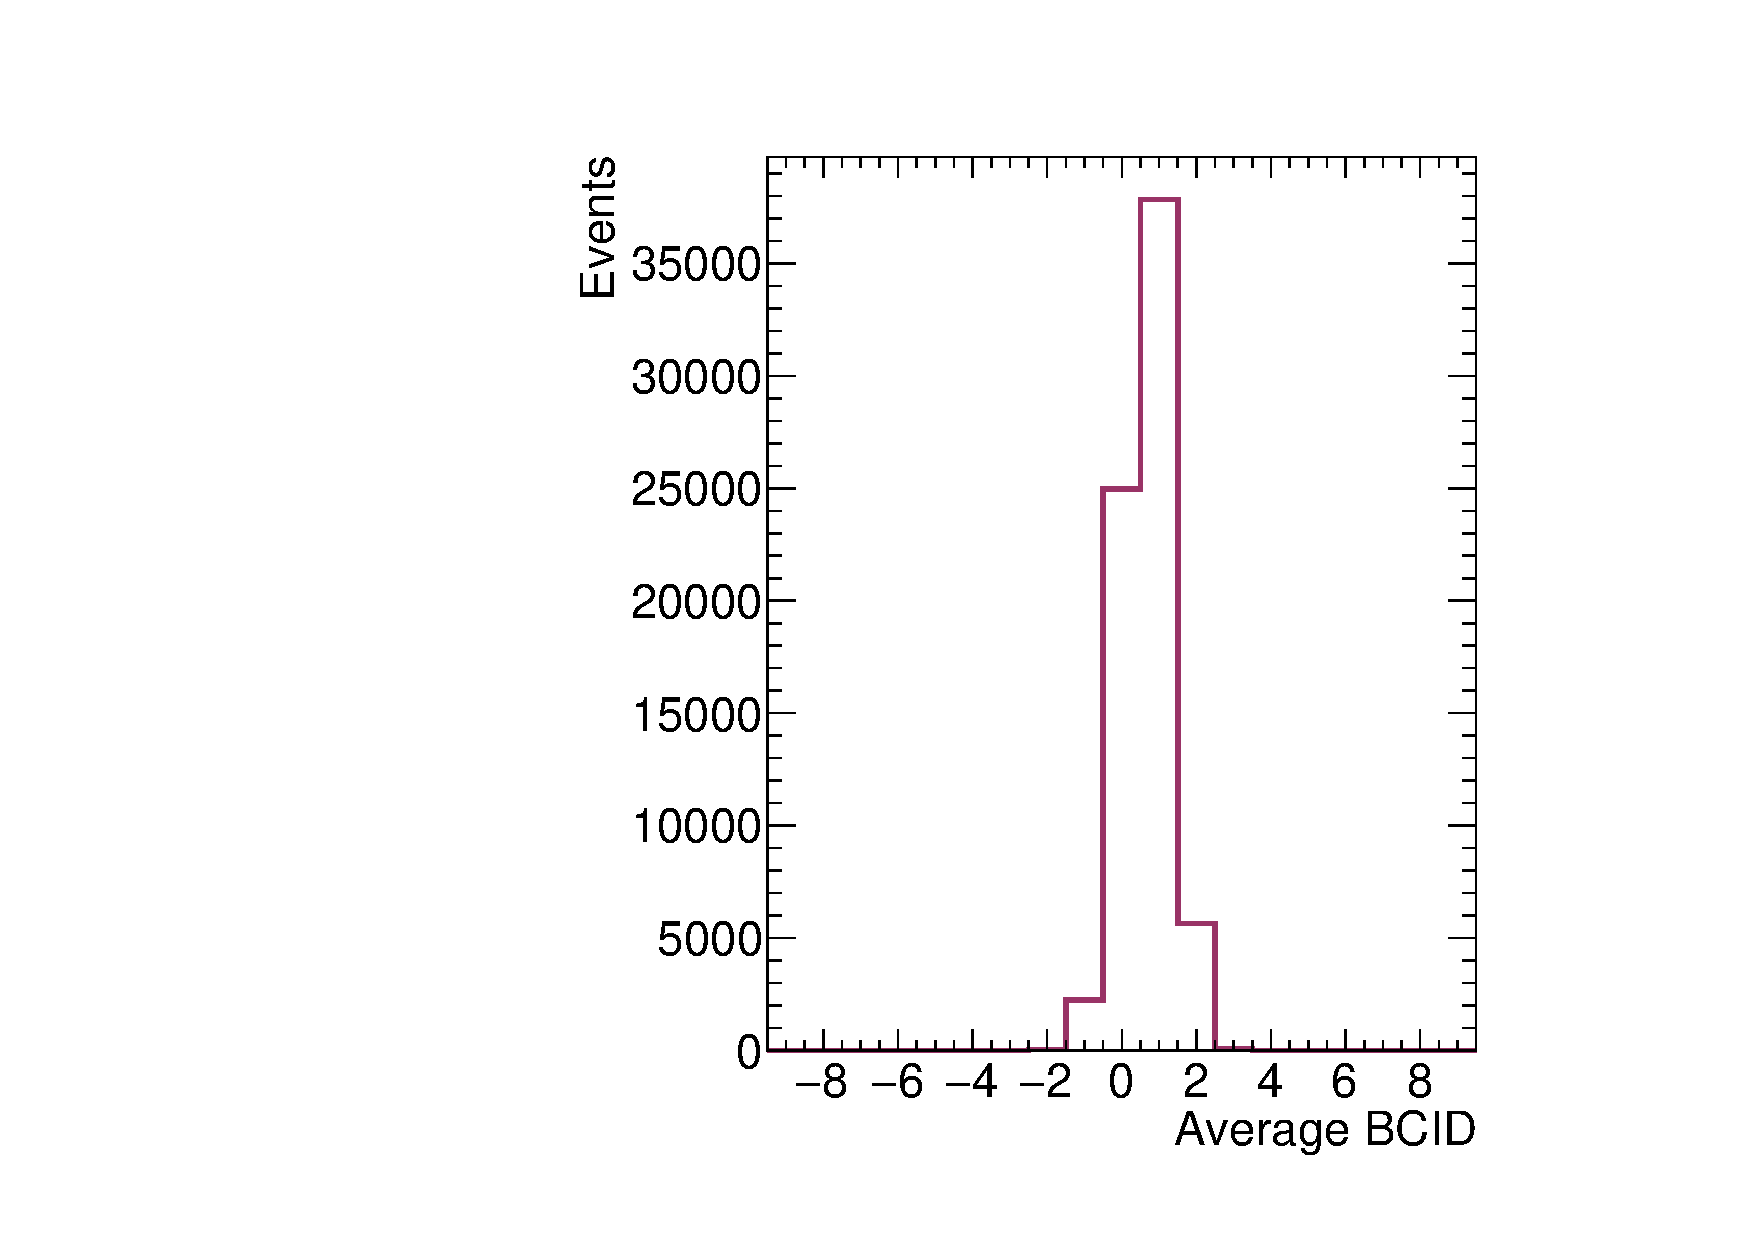
\includegraphics[width=0.3\textwidth]{figures/gbtanalysis3528/avg_BCID.pdf}
  \end{center}
  \vspace{-10pt}
  \caption{The time resolution of the MM TP relative to the scintillator, where the BC of the trigger is defined as the average BCID of the ART hits, for data collected with 200 ns (left), 100 ns (middle), and 50 ns (right) integration time in the VMM.}
  \label{fig:integ_avg_bc}
\end{figure}

\begin{figure}[!htpb]
  \begin{center}
    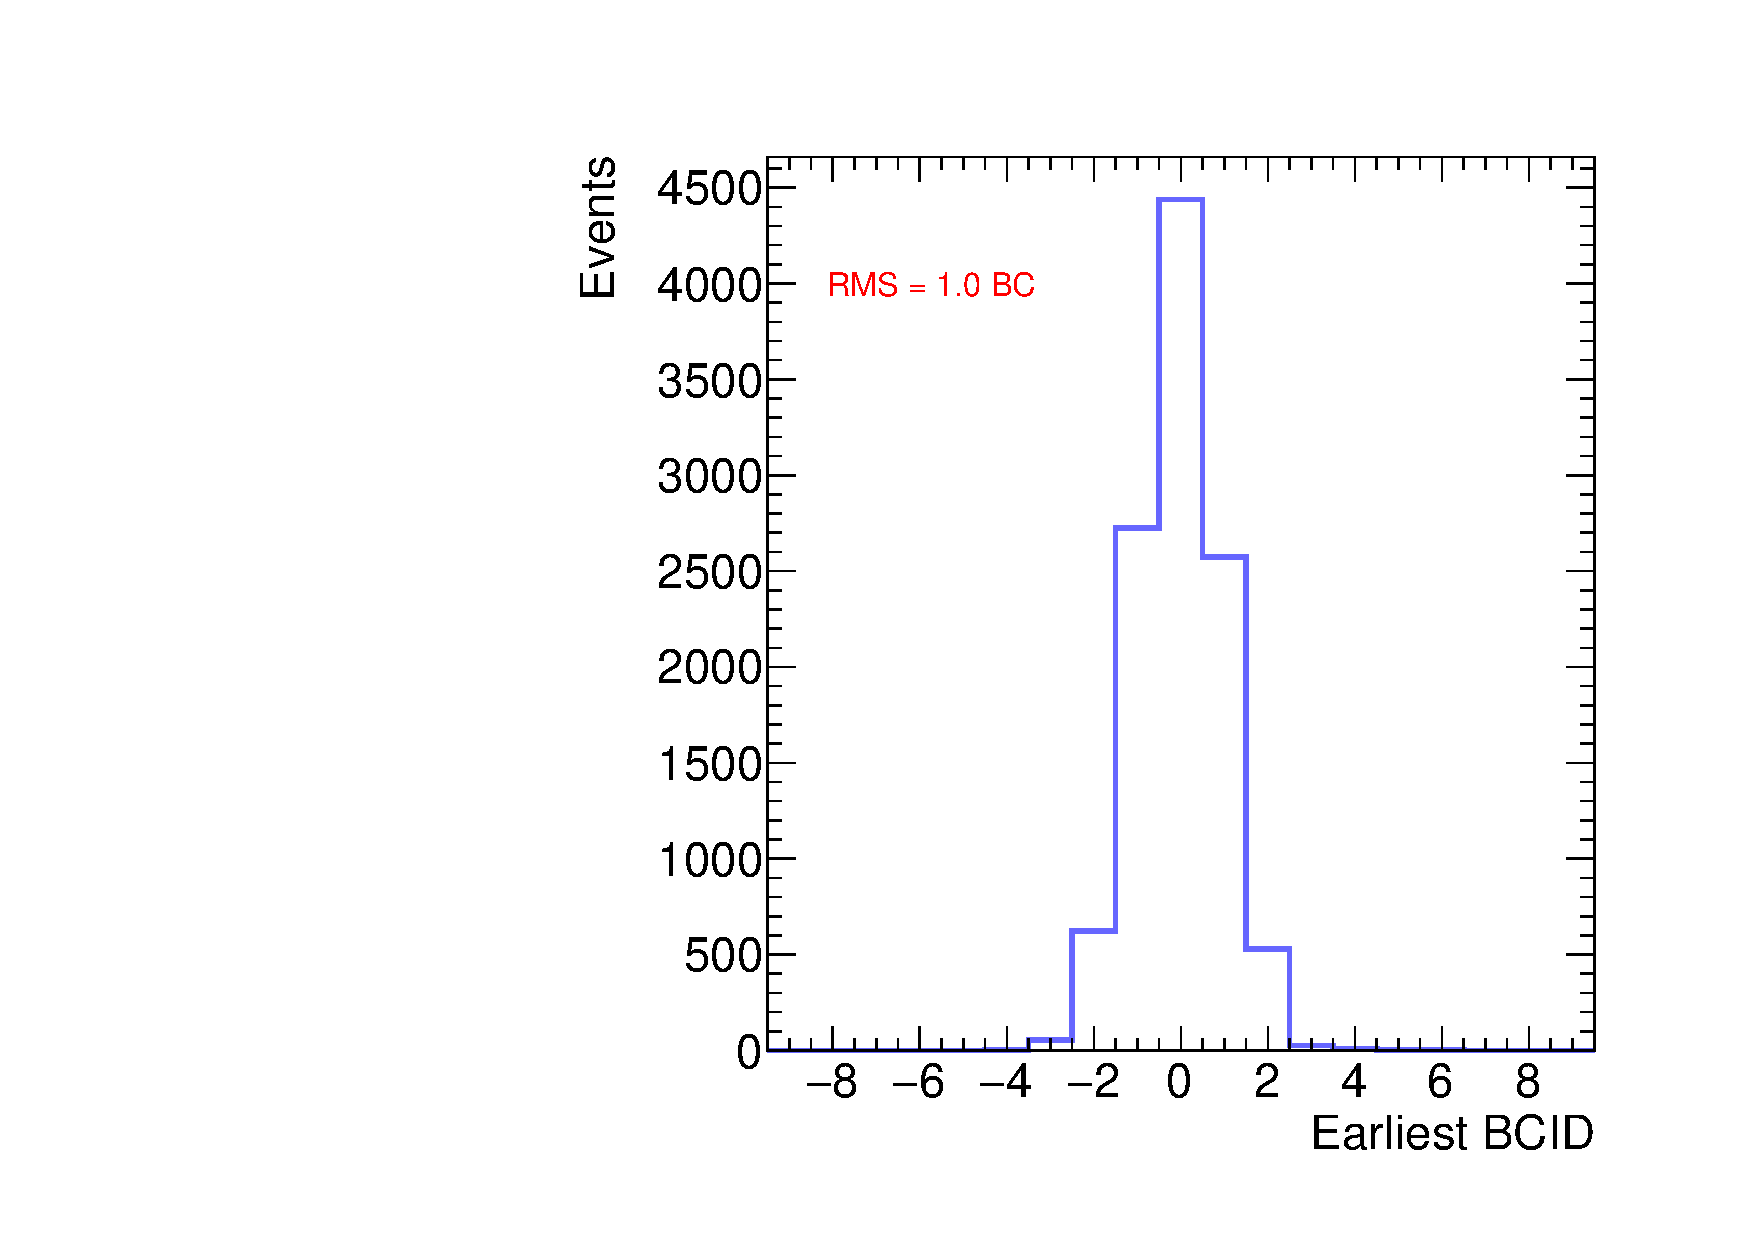
\includegraphics[width=0.3\textwidth]{figures/gbtanalysis3530/earliest_BCID.pdf}
    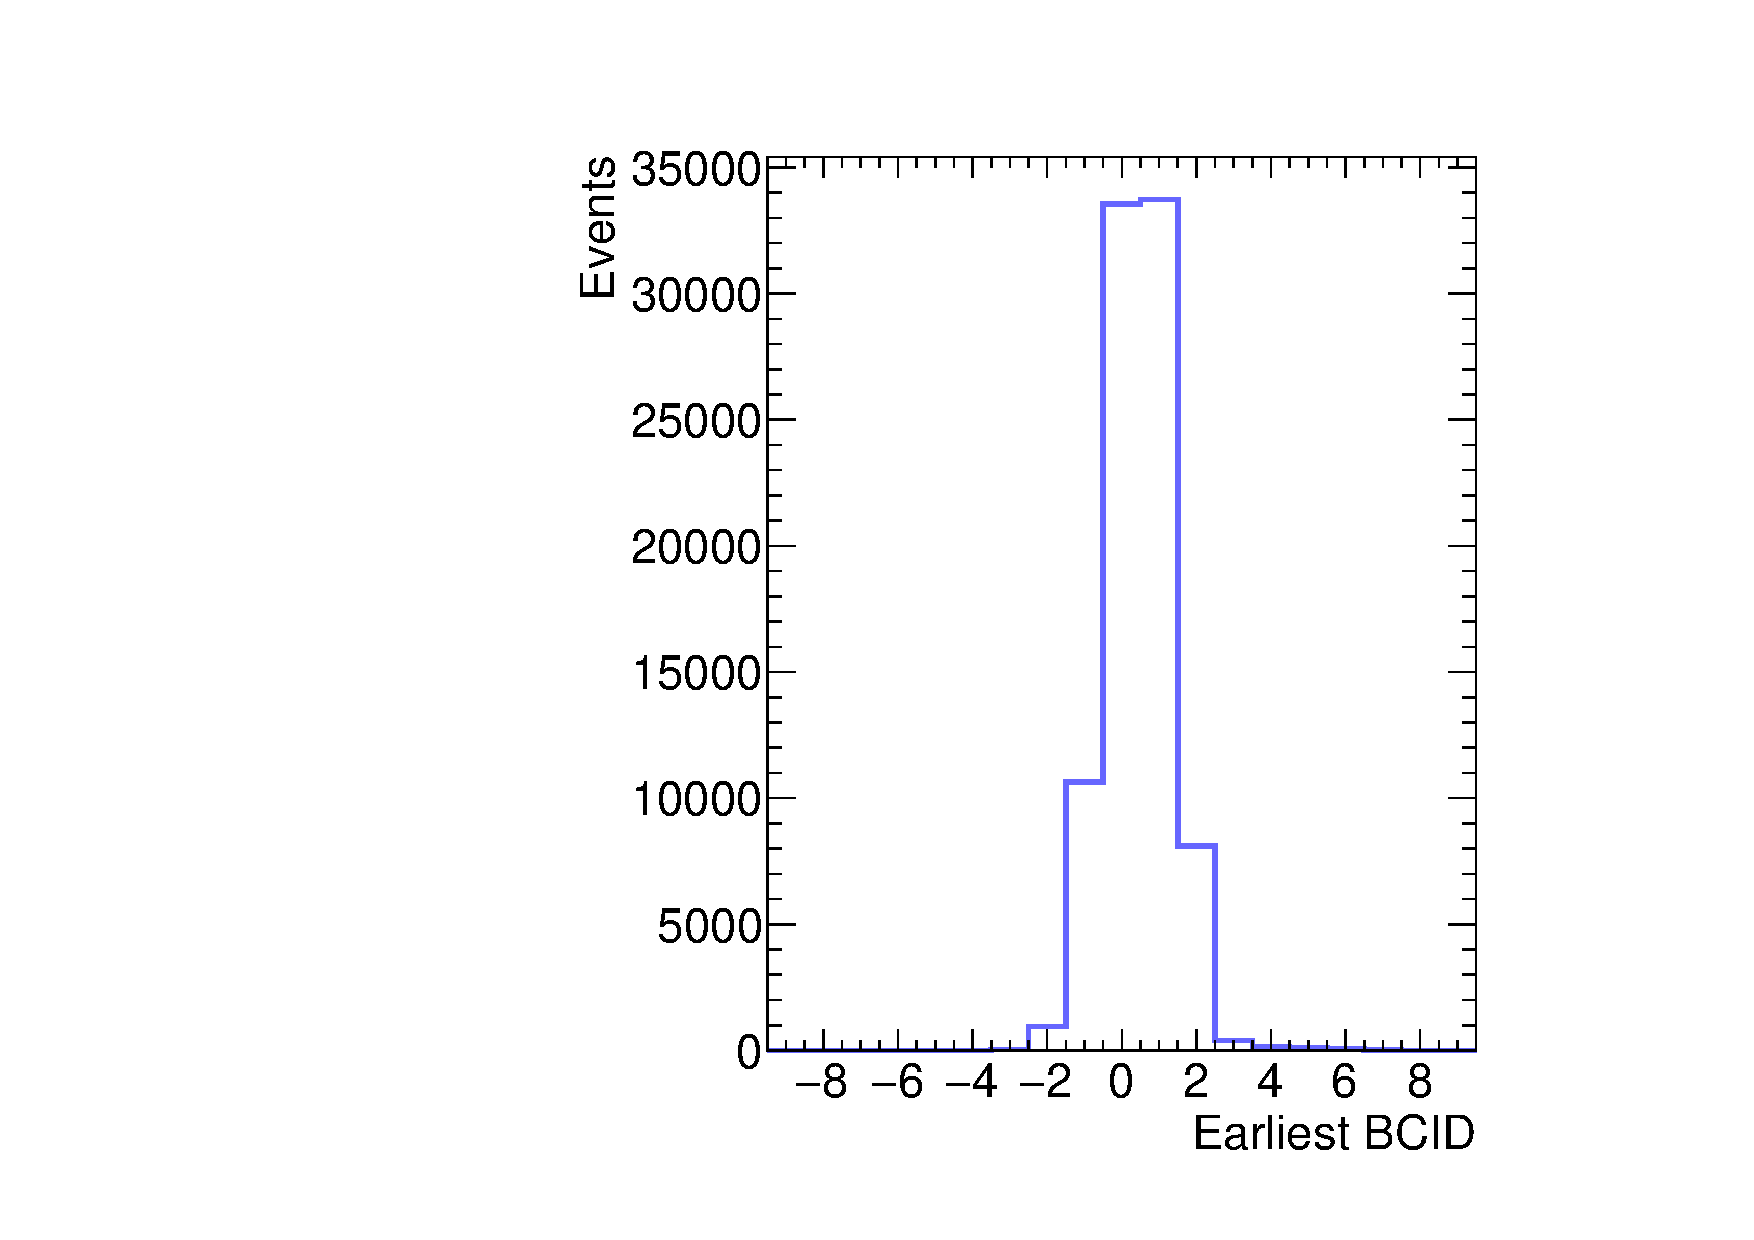
\includegraphics[width=0.3\textwidth]{figures/gbtanalysis3527/earliest_BCID.pdf}
    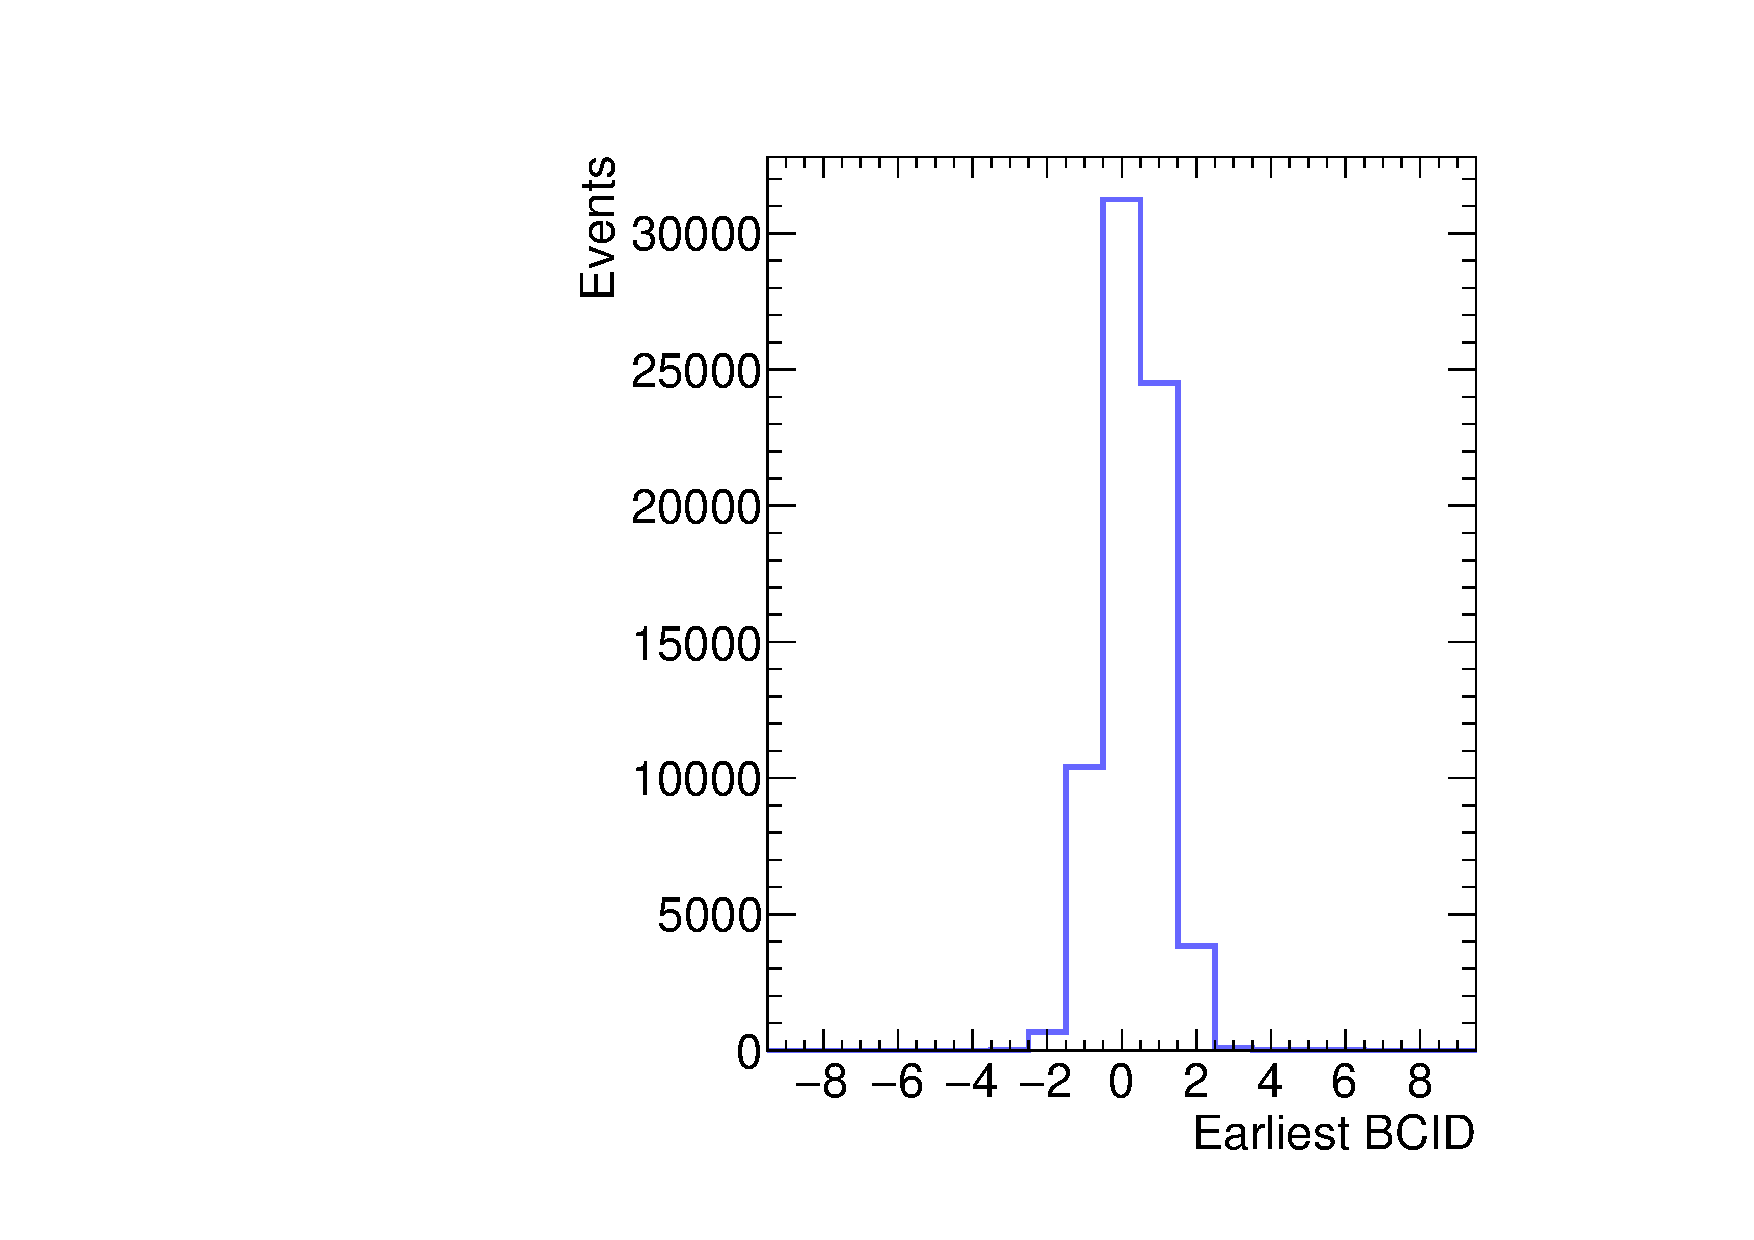
\includegraphics[width=0.3\textwidth]{figures/gbtanalysis3528/earliest_BCID.pdf}
  \end{center}
  \vspace{-10pt}
  \caption{The time resolution of the MM TP relative to the scintillator, where the BC of the trigger is defined as the earliest BCID of the ART hits, for data collected with 200 ns (left), 100 ns (middle), and 50 ns (right) integration time in the VMM.}
  \label{fig:integ_avg_earliest}
\end{figure}


